\documentclass[oneside, UTF8]{ctexbook}

\usepackage{mystyle}
\usepackage{enumitem}
\usepackage{float}
\usepackage{booktabs}

\graphicspath{{figs/}}

\begin{document}

\frontmatter
\pagestyle{plain}

\begin{spacing}{1.2}
  \tableofcontents
\end{spacing}
\newpage

\mainmatter

\setcounter{chapter}{1}
\chapter{系统实现}

本章在概要设计的基础上，对在线商城系统的实际运行环境、开发工具选择以及主要功能实现情况进行说明。系统实现以“客户购买、商家经营、管理员治理”为主要业务线索，围绕商品展示、检索筛选、购物车、订单、支付、物流、后台管理和推荐展示等功能展开。为了保证正文表述符合正式设计报告要求，本章重点说明实现思路、采用技术和页面效果，不展开具体程序代码。

\section{系统配置}

系统采用前后端分离和容器化辅助部署方式运行。前端负责页面展示和交互承接，后端负责业务接口、数据校验、权限控制和持久化访问，数据库与对象存储分别承担结构化业务数据和商品图片等资源文件的保存。系统在开发和测试阶段可以部署在单台计算机上，也可以按照服务边界拆分到多台服务器上运行。

\begin{table}[H]
  \centering
  \caption{系统运行环境配置}
  \label{tab:implementation_system_config}
  \small
  \renewcommand{\arraystretch}{1.22}
  \begin{tabular}{p{0.22\textwidth}p{0.30\textwidth}p{0.34\textwidth}}
    \toprule
    配置类别 & 推荐配置 & 说明 \\
    \midrule
    处理器 & 多核心 x86\_64 处理器 & 支撑前端构建、后端服务和数据库并行运行 \\
    内存 & 16GB 及以上 & 保证数据库、对象存储和开发服务同时运行时保持稳定 \\
    存储空间 & 50GB 及以上可用空间 & 保存项目文件、依赖包、数据库数据和商品图片资源 \\
    操作系统 & Windows 或 Linux 环境 & 开发阶段以 Windows 为主，部署阶段可迁移到 Linux 服务器 \\
    浏览器 & Chrome、Edge 等现代浏览器 & 用于访问商城页面、调试交互效果和验证页面兼容性 \\
    网络环境 & 本地局域网或稳定互联网 & 支撑服务间访问、依赖获取和后续远程部署 \\
    \bottomrule
  \end{tabular}
\end{table}

软件运行环境由应用运行时、数据服务和基础支撑服务组成。前端页面运行在 Node.js 环境中，后端服务运行在 Python 环境中，业务数据保存在 PostgreSQL 中，商品图片和推荐数据文件等资源通过对象存储进行管理。系统还预留 Hadoop 和 Spark 相关服务，用于较大规模行为数据的离线处理和推荐结果计算。

\begin{table}[H]
  \centering
  \caption{系统软件环境配置}
  \label{tab:implementation_software_config}
  \small
  \renewcommand{\arraystretch}{1.22}
  \begin{tabular}{p{0.22\textwidth}p{0.30\textwidth}p{0.34\textwidth}}
    \toprule
    软件类别 & 采用环境 & 作用说明 \\
    \midrule
    前端运行环境 & Node.js 20、Yarn & 支撑商城前端页面开发、构建和运行 \\
    后端运行环境 & Python 3.10 及以上 & 支撑业务接口服务和后端应用逻辑运行 \\
    Web 服务框架 & FastAPI、Uvicorn & 提供高性能接口服务和异步请求处理能力 \\
    数据库 & PostgreSQL 16 & 保存账户、店铺、商品、订单、支付、物流等结构化数据 \\
    对象存储 & MinIO & 保存商品图片、静态资源和数据处理文件 \\
    容器环境 & Docker Compose & 统一编排前端、后端、数据库和对象存储等服务 \\
    推荐处理环境 & Hadoop、Spark & 支撑行为数据整理、批处理计算和推荐结果生成 \\
    \bottomrule
  \end{tabular}
\end{table}

系统运行时主要开放前端访问入口、后端接口入口、数据库服务端口和对象存储服务端口。前端入口用于客户、商家和管理员访问页面；后端入口用于承接前端业务请求；数据库和对象存储主要由后端服务访问，不直接暴露给普通用户。通过这种方式，系统既能满足本地开发调试需要，也能在正式部署时通过访问控制减少数据层暴露范围。

\section{开发工具}

系统开发采用面向工程实践的工具组合。前端开发侧重页面组件组织、响应式布局和用户交互体验；后端开发侧重接口设计、业务规则封装和数据访问；数据库与部署工具侧重数据稳定性、服务可恢复性和运行环境一致性。各类工具之间分工明确，共同支撑系统从设计、开发、调试到部署的完整过程。

\begin{table}[H]
  \centering
  \caption{系统开发工具与技术}
  \label{tab:implementation_dev_tools}
  \small
  \renewcommand{\arraystretch}{1.22}
  \begin{tabular}{p{0.22\textwidth}p{0.30\textwidth}p{0.34\textwidth}}
    \toprule
    工具类别 & 主要工具或技术 & 用途说明 \\
    \midrule
    前端框架 & Next.js、React、TypeScript & 构建商城页面、角色入口和交互组件 \\
    样式与组件 & Tailwind CSS、Medusa UI、Headless UI & 实现页面布局、按钮表单、筛选面板和交互控件 \\
    后端框架 & FastAPI、Pydantic、Uvicorn & 实现接口服务、数据校验和请求响应处理 \\
    数据访问 & SQLAlchemy、asyncpg & 实现异步数据库访问和业务数据持久化 \\
    对象存储访问 & MinIO 客户端 & 支撑商品图片、资源文件和数据文件管理 \\
    身份与安全 & 密码散列、令牌校验、角色权限控制 & 支撑客户、商家和管理员的身份识别与权限隔离 \\
    开发协作 & Git、终端工具、浏览器调试工具 & 支撑版本管理、服务启动、日志查看和页面验证 \\
    文档制图 & PlantUML、Graphviz、LaTeX & 支撑架构图、模块图、时序图、E-R 图和报告排版 \\
    \bottomrule
  \end{tabular}
\end{table}

前端技术选择以组件化和页面组织能力为重点。Next.js 负责页面路由、服务端数据获取和页面构建，React 负责组件状态和界面复用，TypeScript 用于提高数据结构表达的清晰度。Tailwind CSS 和相关 UI 组件库用于统一按钮、表单、导航、筛选条件和商品卡片等界面元素，使系统在不同页面之间保持一致的交互风格。

后端技术选择以接口清晰、校验严格和扩展方便为重点。FastAPI 适合构建结构化接口，Pydantic 用于请求参数和响应数据校验，Uvicorn 提供异步服务运行能力。数据库访问采用异步方式，能够在商品浏览、购物车更新、订单提交和后台查询等场景中保持较好的响应能力。对象存储与数据库分离，可以避免把图片文件直接放入数据库，提高资源管理的灵活性。

部署与调试工具选择以环境一致性为重点。Docker Compose 将前端、后端、数据库、对象存储以及推荐处理相关服务组织在统一网络中，便于本地复现完整运行环境。浏览器调试工具用于检查页面渲染、网络请求和交互状态；服务日志用于定位接口异常、数据异常和部署异常。文档制作过程中使用 LaTeX 统一正文格式，并通过图表展示系统结构和实现效果。

\section{功能实现}

系统功能实现按照业务模块展开。客户侧重点是浏览、筛选、购买和查看订单；商家侧重点是店铺经营、商品维护和订单处理；管理员侧重点是平台审核、用户管理和运行治理。各功能模块通过统一的服务入口访问后端接口，再由后端完成业务校验、数据读写和状态变更。

\subsection{客户商品浏览与推荐展示}

客户进入商城后首先看到首页展示区域。首页承担商品曝光、推荐引导、搜索入口和分类筛选入口等职责，是客户购物流程的起点。实现时，前端页面先向后端获取商品列表、推荐商品、店铺信息和分类信息，再将这些数据组织为推荐区域、搜索区域、筛选区域和商品信息流。这样既能突出推荐商品，也能让客户快速进入指定分类或店铺。

\begin{figure}[H]
  \centering
  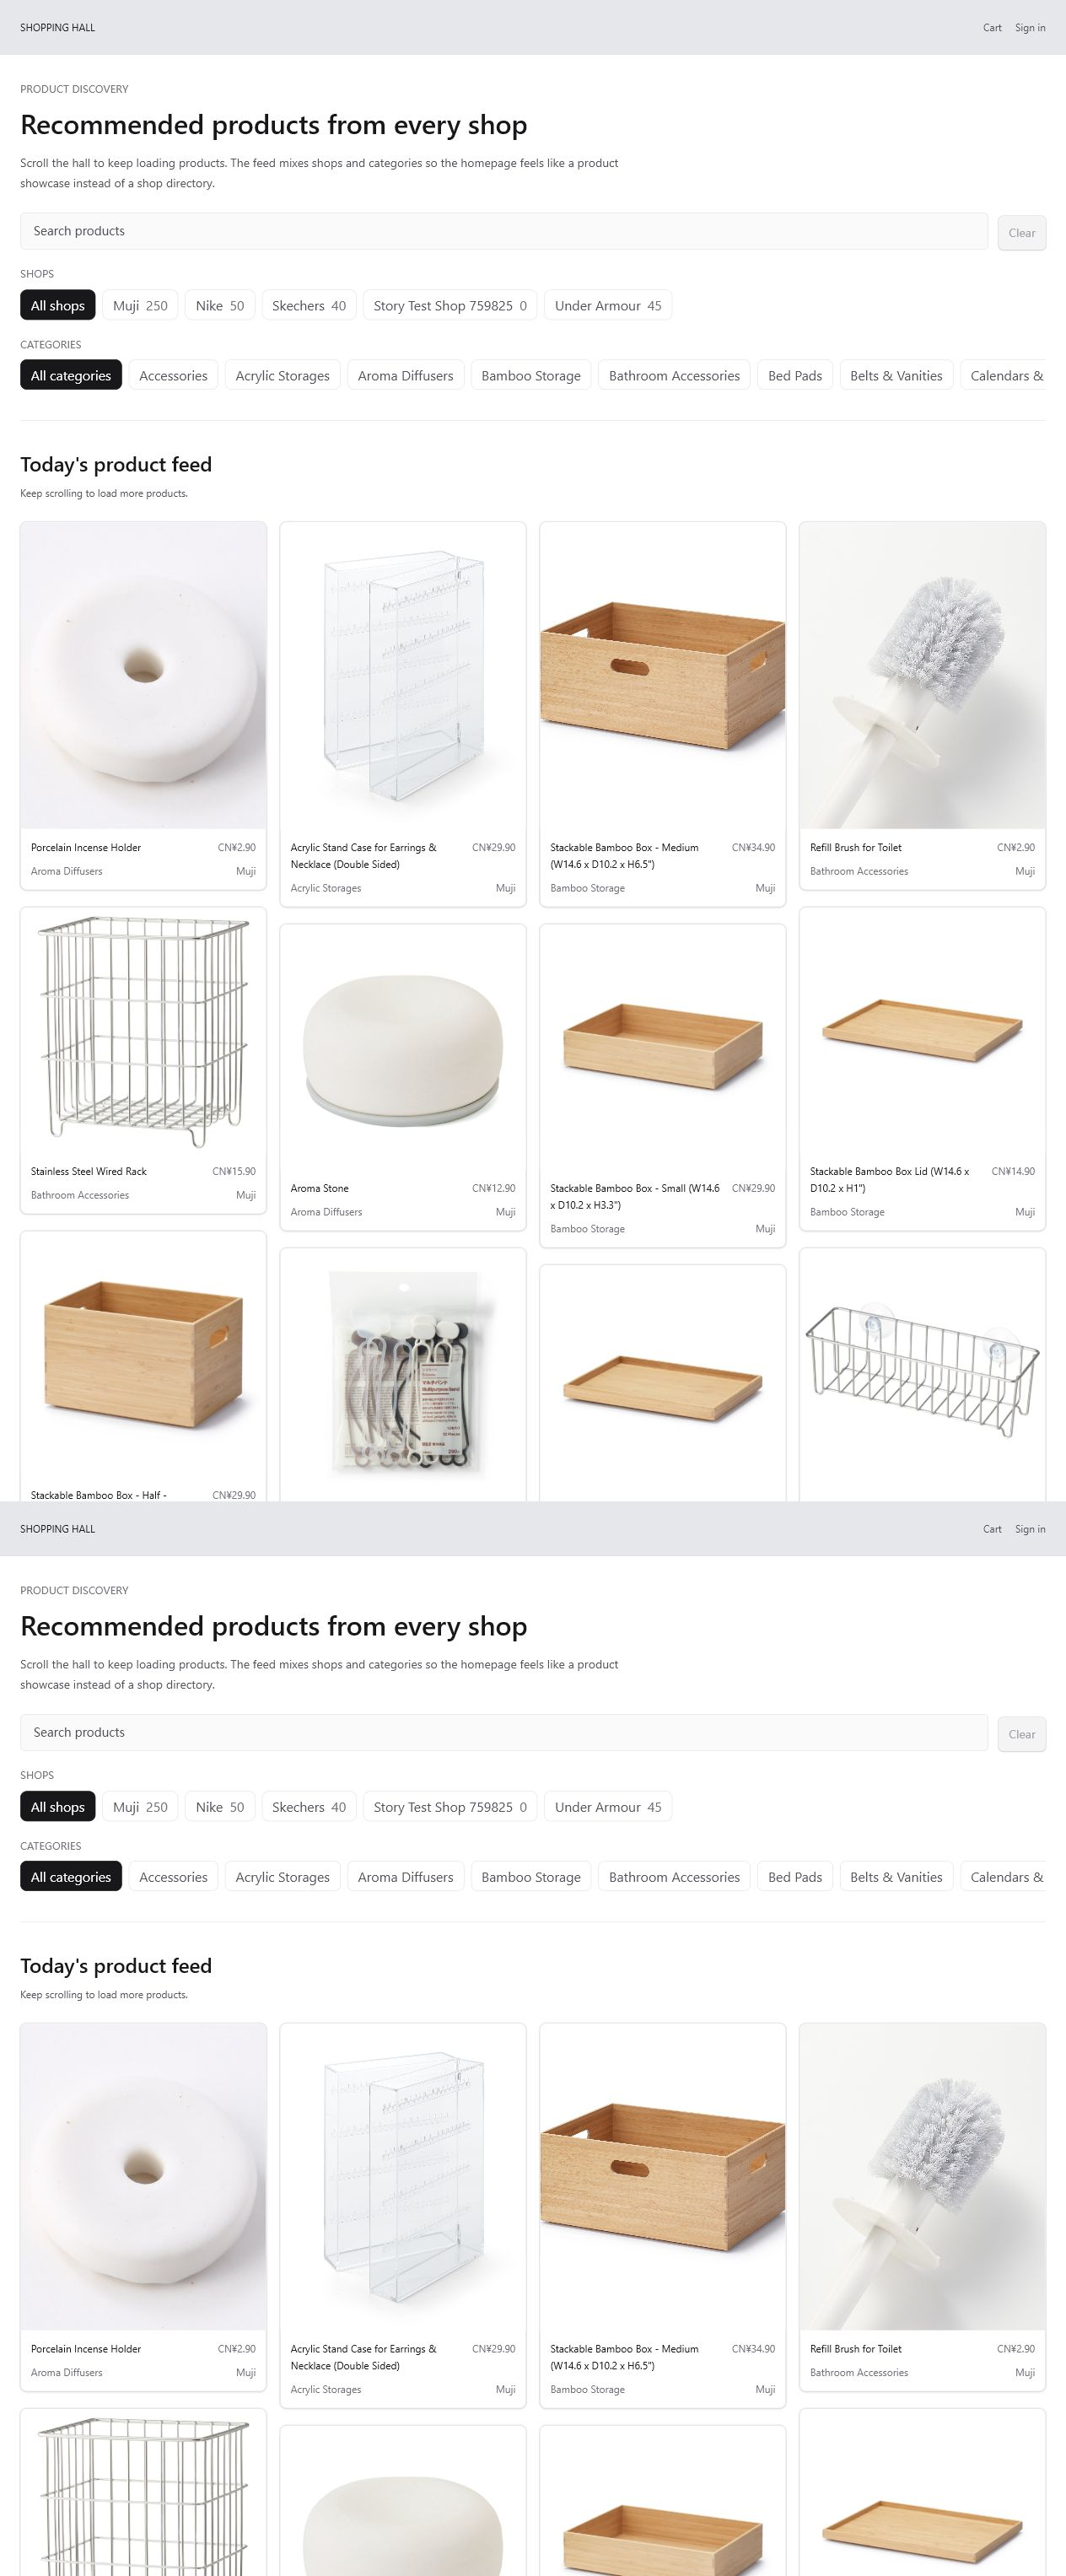
\includegraphics[width=0.92\textwidth,height=0.76\textheight,keepaspectratio]{implementation-home-long.png}
  \caption{商城首页与推荐展示效果}
  \label{fig:implementation_home}
\end{figure}

图 \ref{fig:implementation_home} 展示了商城首页的实际效果。页面上方保留统一导航入口，中部展示推荐商品和搜索筛选能力，下方以商品卡片形式展示商品信息。商品卡片将图片、名称、价格、店铺和进入详情的操作集中呈现，便于客户快速比较。推荐展示不直接影响下单链路，即使推荐数据暂时不可用，系统仍可通过普通商品列表保证客户完成浏览和购买。

\subsection{商品列表与筛选排序}

商品列表模块负责承接客户的主动浏览需求。该模块通过分类、店铺、价格、关键字和排序条件缩小商品范围，并以统一卡片布局展示查询结果。实现时，前端将客户选择的筛选条件整理为查询参数，后端根据参数进行数据检索、状态过滤和结果排序，最后返回符合条件的商品集合。

\begin{figure}[H]
  \centering
  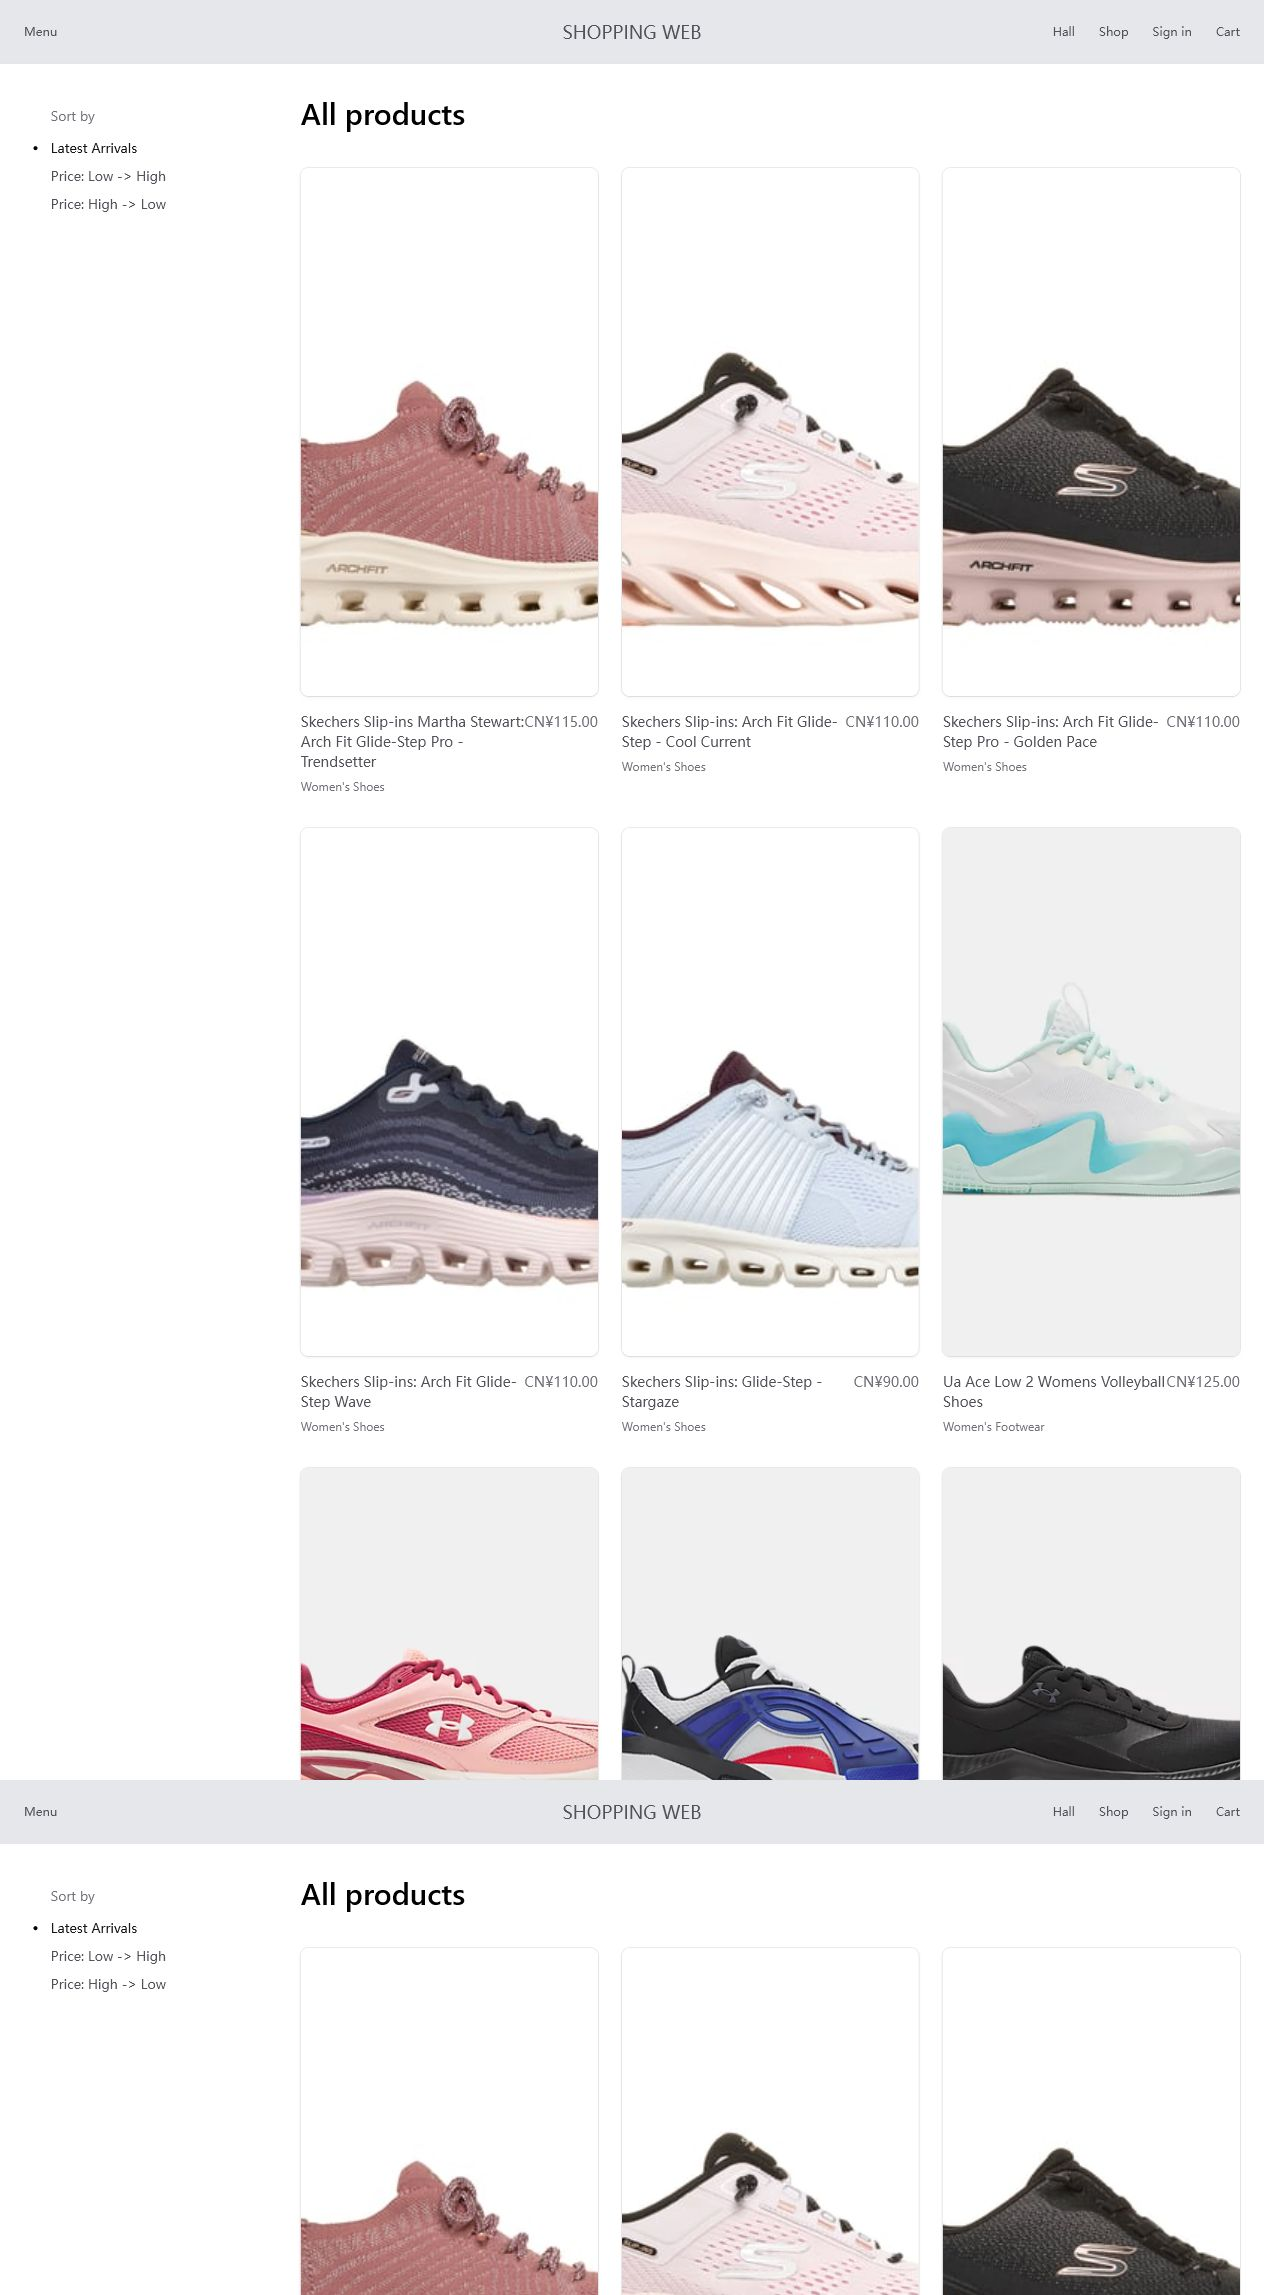
\includegraphics[width=0.92\textwidth,height=0.76\textheight,keepaspectratio]{implementation-shop-long.png}
  \caption{商品列表与筛选排序效果}
  \label{fig:implementation_shop}
\end{figure}

图 \ref{fig:implementation_shop} 展示了商品列表页面的实际效果。页面左侧提供排序和筛选入口，右侧展示商品网格。列表实现的重点是保持筛选条件、分页结果和页面状态一致：当客户修改排序方式或筛选条件时，页面应重新获取匹配结果；当客户进入商品详情后返回列表时，应尽量保留原有浏览上下文。该模块为后续下单、收藏和推荐反馈提供基础入口。

\subsection{购物车与订单结算}

购物车模块用于保存客户尚未提交的购买意向。客户可以从商品详情或商品列表中选择商品加入购物车，并在购物车中调整数量、删除商品或进入结算流程。实现时，购物车数据与客户账户关联，购物车明细保存商品、规格、数量和价格等信息。后端在更新购物车时需要校验商品状态、库存状态和数量有效性，避免无效商品进入结算流程。

\begin{figure}[H]
  \centering
  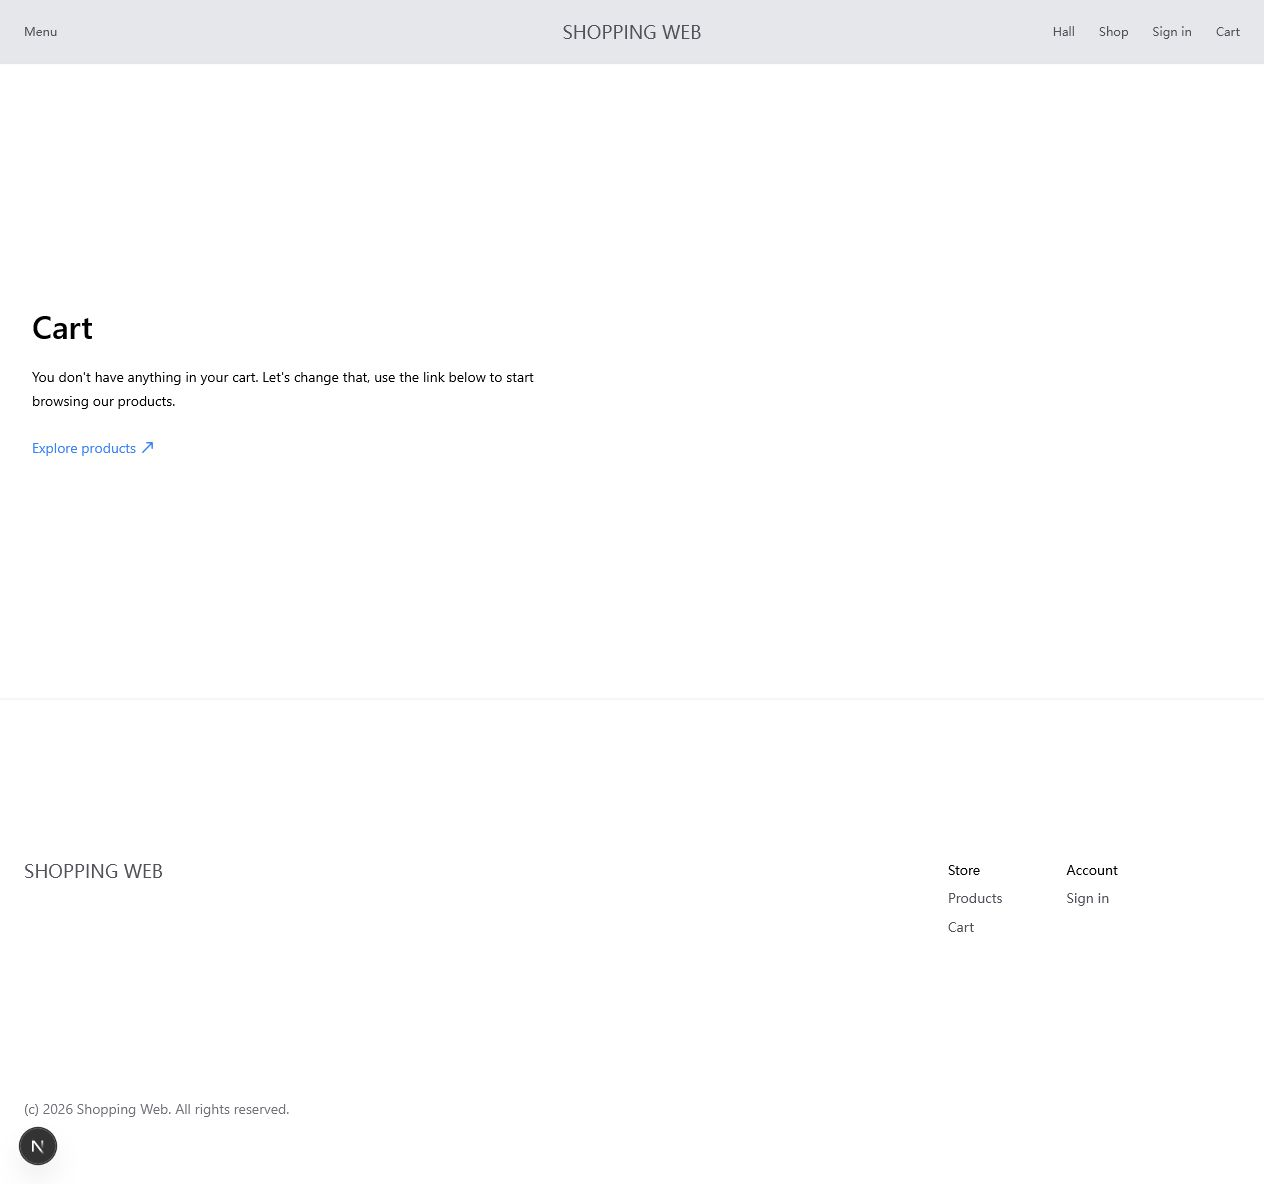
\includegraphics[width=0.92\textwidth,height=0.76\textheight,keepaspectratio]{implementation-cart-long.png}
  \caption{购物车页面展示效果}
  \label{fig:implementation_cart}
\end{figure}

图 \ref{fig:implementation_cart} 展示了购物车为空时的页面状态。购物车不仅需要展示已有商品，也需要处理空购物车、商品失效、数量超限和价格变化等边界情况。订单结算时，系统根据购物车明细生成订单主信息和订单明细，并进入支付与履约流程。订单生成后，订单明细应保存当时的购买信息，避免后续商品价格或名称变化影响历史订单。

\subsection{角色登录与权限入口}

系统面向客户、商家和管理员三类角色，因此登录模块不仅负责身份认证，也负责角色入口划分。登录页面提供不同角色的选择入口，客户登录后进入购物相关页面，商家登录后进入店铺经营页面，管理员登录后进入平台治理页面。后端根据账户信息、角色标识和状态进行校验，前端根据校验结果引导用户进入对应功能范围。

\begin{figure}[H]
  \centering
  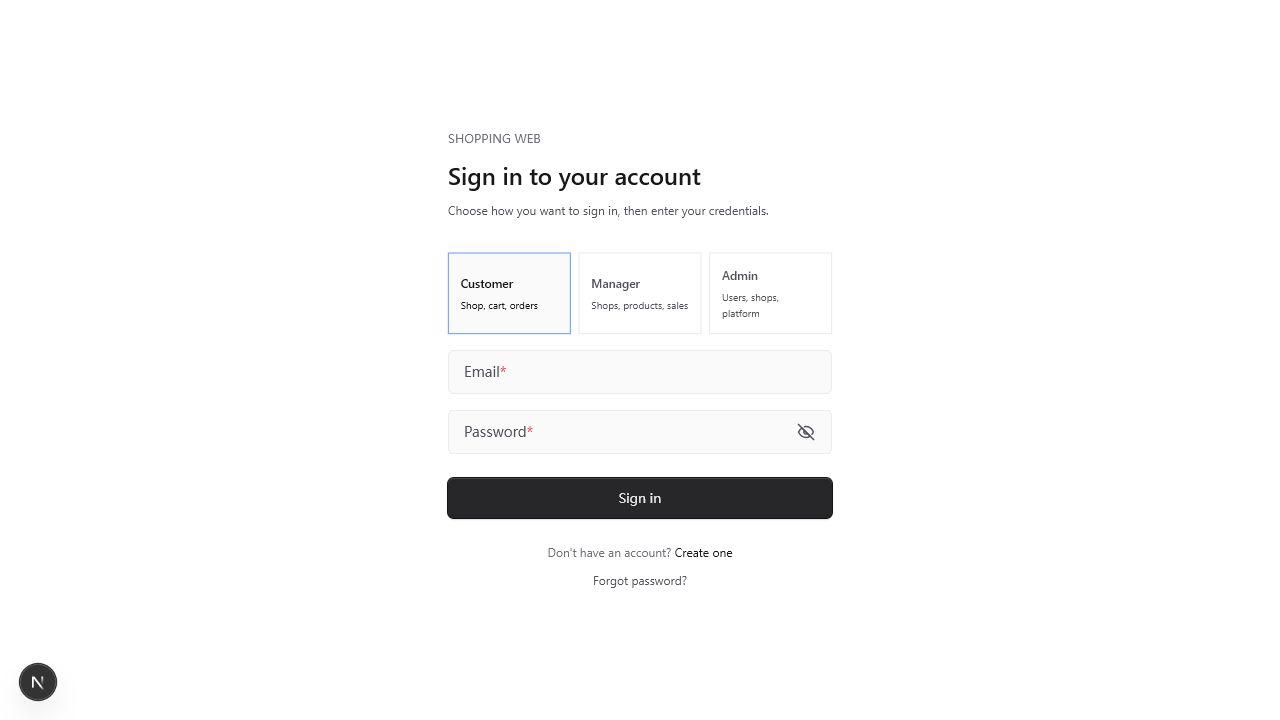
\includegraphics[width=0.86\textwidth,height=0.72\textheight,keepaspectratio]{implementation-login-long.png}
  \caption{三类角色登录入口效果}
  \label{fig:implementation_login}
\end{figure}

图 \ref{fig:implementation_login} 展示了统一登录页面。该页面通过角色选项明确区分客户、商家和管理员入口，降低用户误操作概率。权限控制的实现重点是保证“登录成功”和“可访问资源”不是同一个概念：客户不能访问商家经营数据，商家不能维护其他店铺商品，管理员操作也应限定在平台管理职责范围内。通过角色隔离，系统能够减少越权访问风险。

\subsection{商家后台与商品维护}

商家后台围绕店铺经营展开，主要包括店铺资料维护、商品上架与下架、商品图片维护、库存与价格调整以及订单处理。实现时，商家账户与店铺建立绑定关系，商家只能维护自己店铺下的商品和订单。商品维护流程通常包括填写商品基本信息、选择分类、上传图片、设置价格和库存、提交保存等步骤。后端在保存商品时需要校验店铺归属、字段完整性和商品状态。

商品维护模块与客户展示模块之间存在直接关系。商家发布或修改商品后，客户侧商品列表和详情页需要能够展示最新有效数据；若商品被下架或审核未通过，客户侧不应继续展示为可购买状态。订单处理模块则要求商家能够查看与本店铺相关的订单明细，完成发货、更新物流和处理异常订单等操作。通过将商家权限限制在店铺范围内，系统能够在支持多店铺经营的同时保持数据边界清晰。

\subsection{管理员审核与平台治理}

管理员模块负责平台级治理，主要包括账户管理、店铺审核、商品审核、异常内容处理和运行状态查看等功能。管理员与商家的区别在于，管理员不直接参与单个店铺经营，而是从平台整体角度维护业务秩序。实现时，管理员操作需要经过身份校验和权限判断，对审核、禁用、恢复等关键操作保留必要记录。

审核流程一般包括待审核数据查询、详情核对、审核结果提交和状态更新。以商品审核为例，管理员查看商家提交的商品信息和图片资源，判断是否符合平台规范，然后将商品状态更新为通过或驳回。通过后商品进入客户可见范围，驳回后商家需要修改后再次提交。该流程体现了后台治理对前台展示的控制作用，也保证平台商品质量和用户体验。

\subsection{推荐数据处理与结果回写}

推荐模块以客户行为数据为基础，围绕浏览、收藏、购物车、订单和评价等行为生成推荐依据。实现时，系统先在业务过程中记录用户行为，再将行为数据整理为可计算的数据集合，随后通过批处理任务计算热门商品、相似商品或个性化推荐结果。计算完成后，推荐结果写回数据库或缓存表，供首页和商品详情页读取展示。

推荐数据处理与核心交易流程保持相对独立。客户下单、支付和查看订单不依赖推荐计算实时完成，因此推荐任务可以采用异步或批处理方式运行。这样既能降低推荐计算对交易链路的影响，又能在后续扩展更复杂算法时保持系统稳定。推荐结果展示时还需要设置兜底策略，当个性化结果不足时，可以展示热门商品或同类商品，保证页面内容完整。

\subsection{数据持久化与对象存储}

系统数据持久化以 PostgreSQL 为核心，保存账户、店铺、商品、购物车、订单、支付、物流、评价和推荐结果等结构化数据。数据库设计强调主键唯一、外键完整、状态受控和时间可追踪。对于订单、支付和物流等关键业务数据，系统需要保证状态变更有明确顺序，避免出现支付记录无法对应订单、订单没有明细或物流记录缺失等问题。

商品图片和部分数据文件通过对象存储管理。对象存储适合保存图片、附件和批处理文件，能够减轻数据库负担。商品表中保存图片资源引用，实际文件由对象存储提供访问能力。这样在商品图片数量增加时，系统可以通过对象存储扩展容量和访问能力，而不需要改变核心业务表结构。数据库与对象存储协同工作，共同支撑商品展示、后台维护和推荐数据处理。

\subsection{部署运行与服务协同}

系统部署时将前端、后端、数据库、对象存储和推荐处理服务组织为相互协作的运行单元。前端服务提供用户访问页面，后端服务提供业务接口，数据库保存结构化数据，对象存储保存资源文件，推荐处理服务定期生成推荐结果。各服务之间通过明确的网络地址和环境配置进行连接，避免把运行参数写死在业务逻辑中。

服务协同的关键是启动顺序和健康检查。数据库和对象存储应先于后端服务可用，后端服务稳定后前端页面才能完整访问业务接口。对于正式部署，还应关注日志记录、异常恢复、数据备份和访问权限。通过容器化编排，系统可以较方便地在不同环境中复现服务组合，减少“开发环境可用、部署环境不可用”的问题。

\subsection{页面流程与状态变化展示}

为了更直观地说明系统功能实现效果，本节进一步按照用户可进入页面补充长截图说明。截图覆盖客户侧浏览入口、商品检索前后状态、店铺聚合、分类聚合、购物车状态、账户入口、注册与找回密码、客户中心入口以及商家经营概览等页面。每张截图均来自系统实际运行页面，能够反映页面结构、数据展示方式和操作前后状态变化。

商城首页是客户进入系统后最先接触的综合页面。页面顶部提供主要导航，主体区域展示推荐商品、搜索输入框、店铺筛选、分类筛选和商品信息流。与普通商品列表相比，首页更强调引导性：客户可以从推荐商品直接进入购买路径，也可以通过搜索和筛选逐步缩小浏览范围。首页长截图如图 \ref{fig:implementation_home_long_extra} 所示。

\begin{figure}[H]
  \centering
  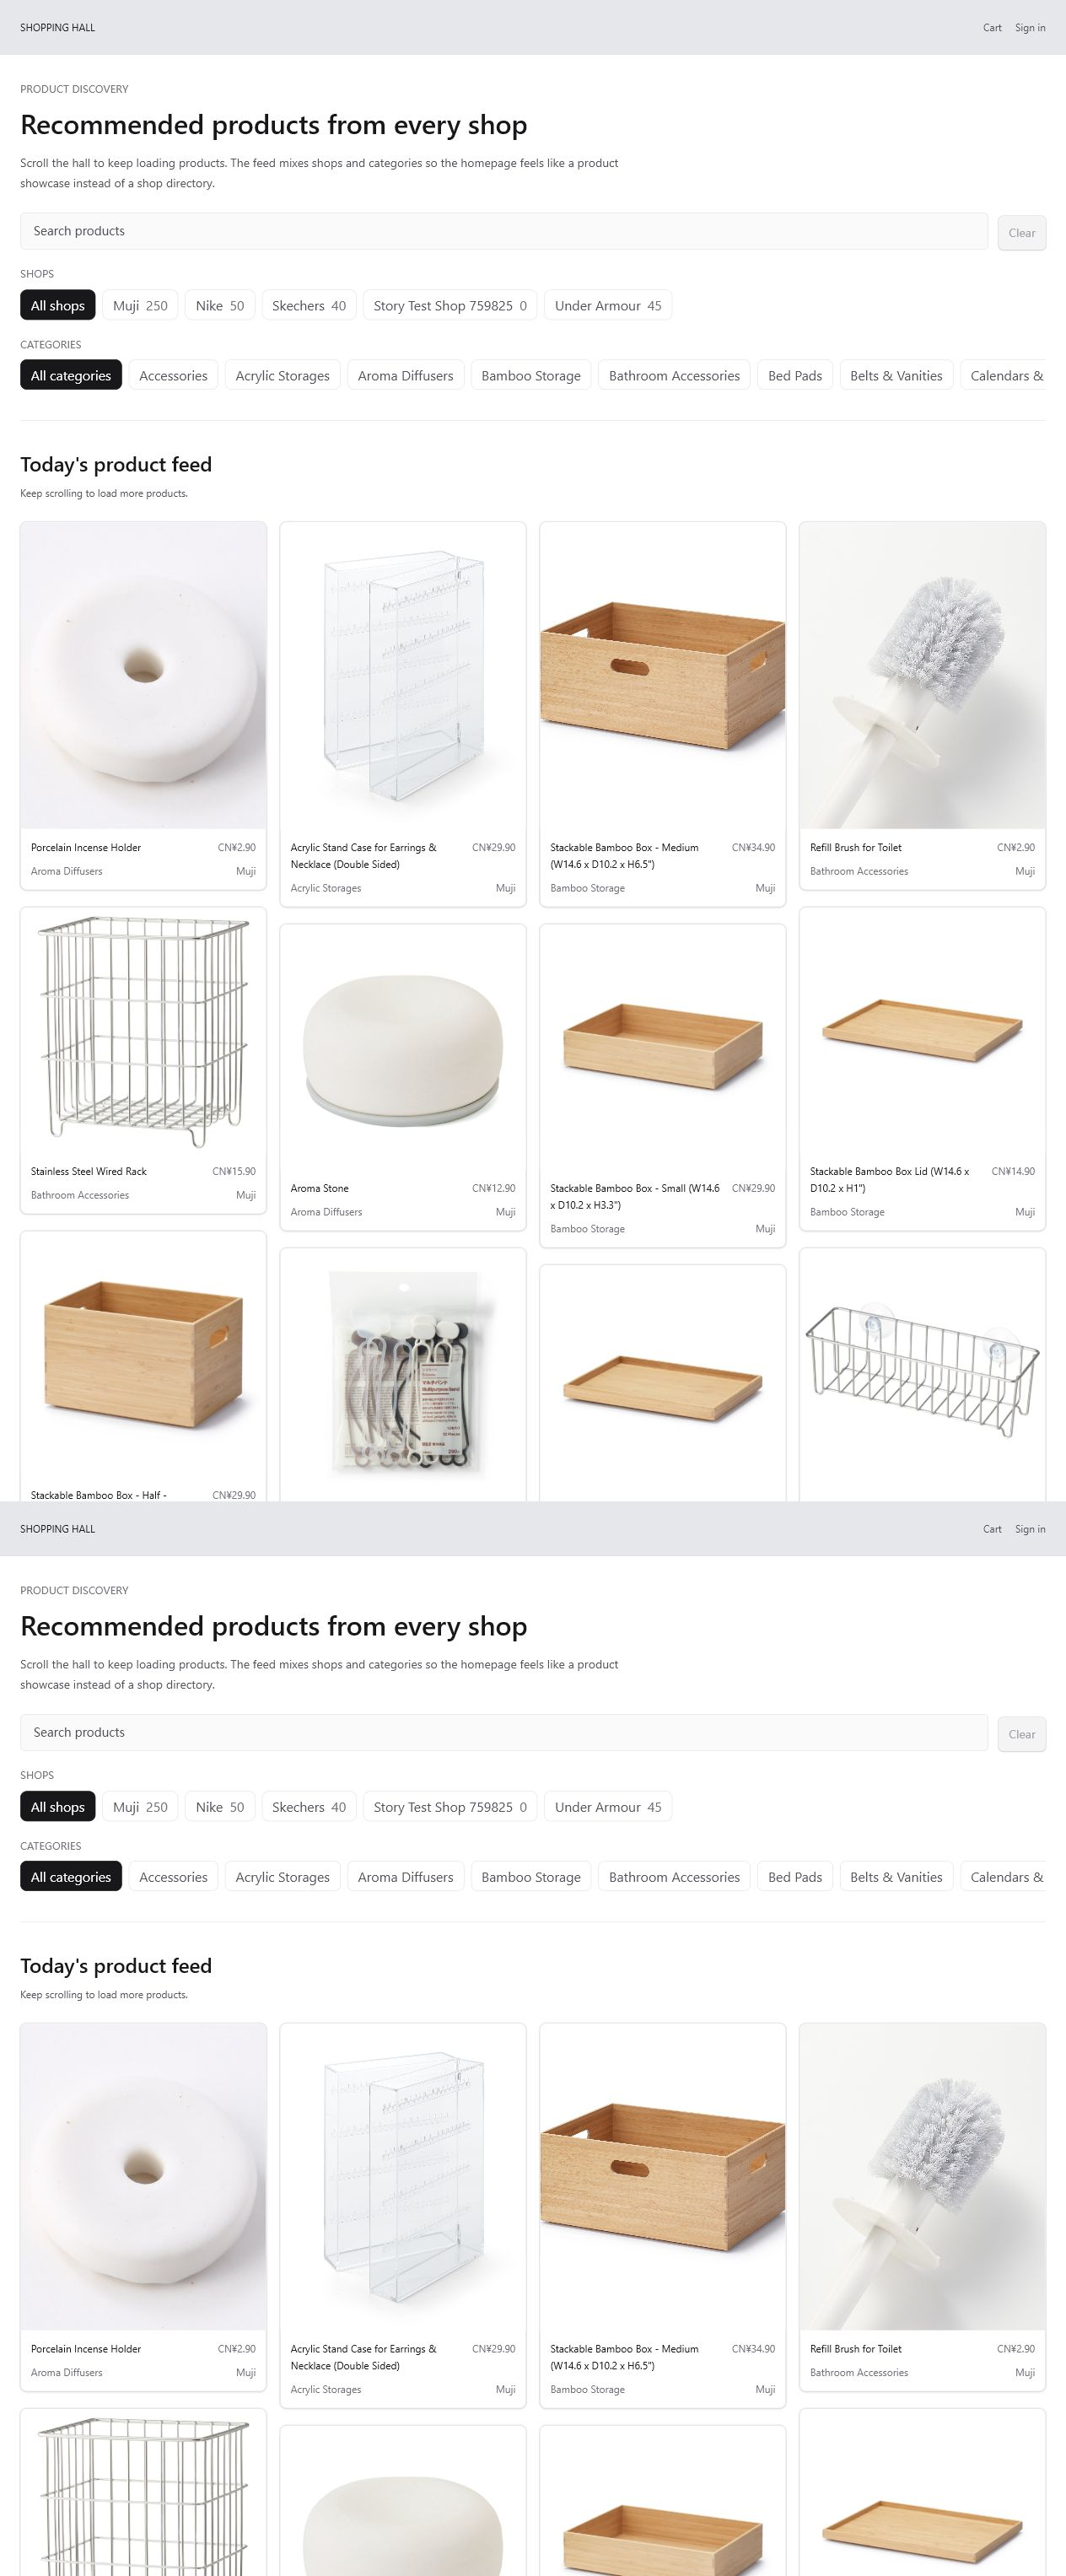
\includegraphics[width=0.92\textwidth,height=0.76\textheight,keepaspectratio]{implementation-home-long.png}
  \caption{商城首页长截图}
  \label{fig:implementation_home_long_extra}
\end{figure}

商品列表页是客户主动查找商品的主要页面。初始状态下，页面展示全部可售商品，并在左侧提供排序条件，右侧以卡片形式展示商品图片、名称、价格和入口。该页面的实现重点是让筛选条件、查询结果和展示布局保持一致，避免客户在多次切换条件时丢失浏览线索。商品列表初始状态如图 \ref{fig:implementation_shop_long_extra} 所示。

\begin{figure}[H]
  \centering
  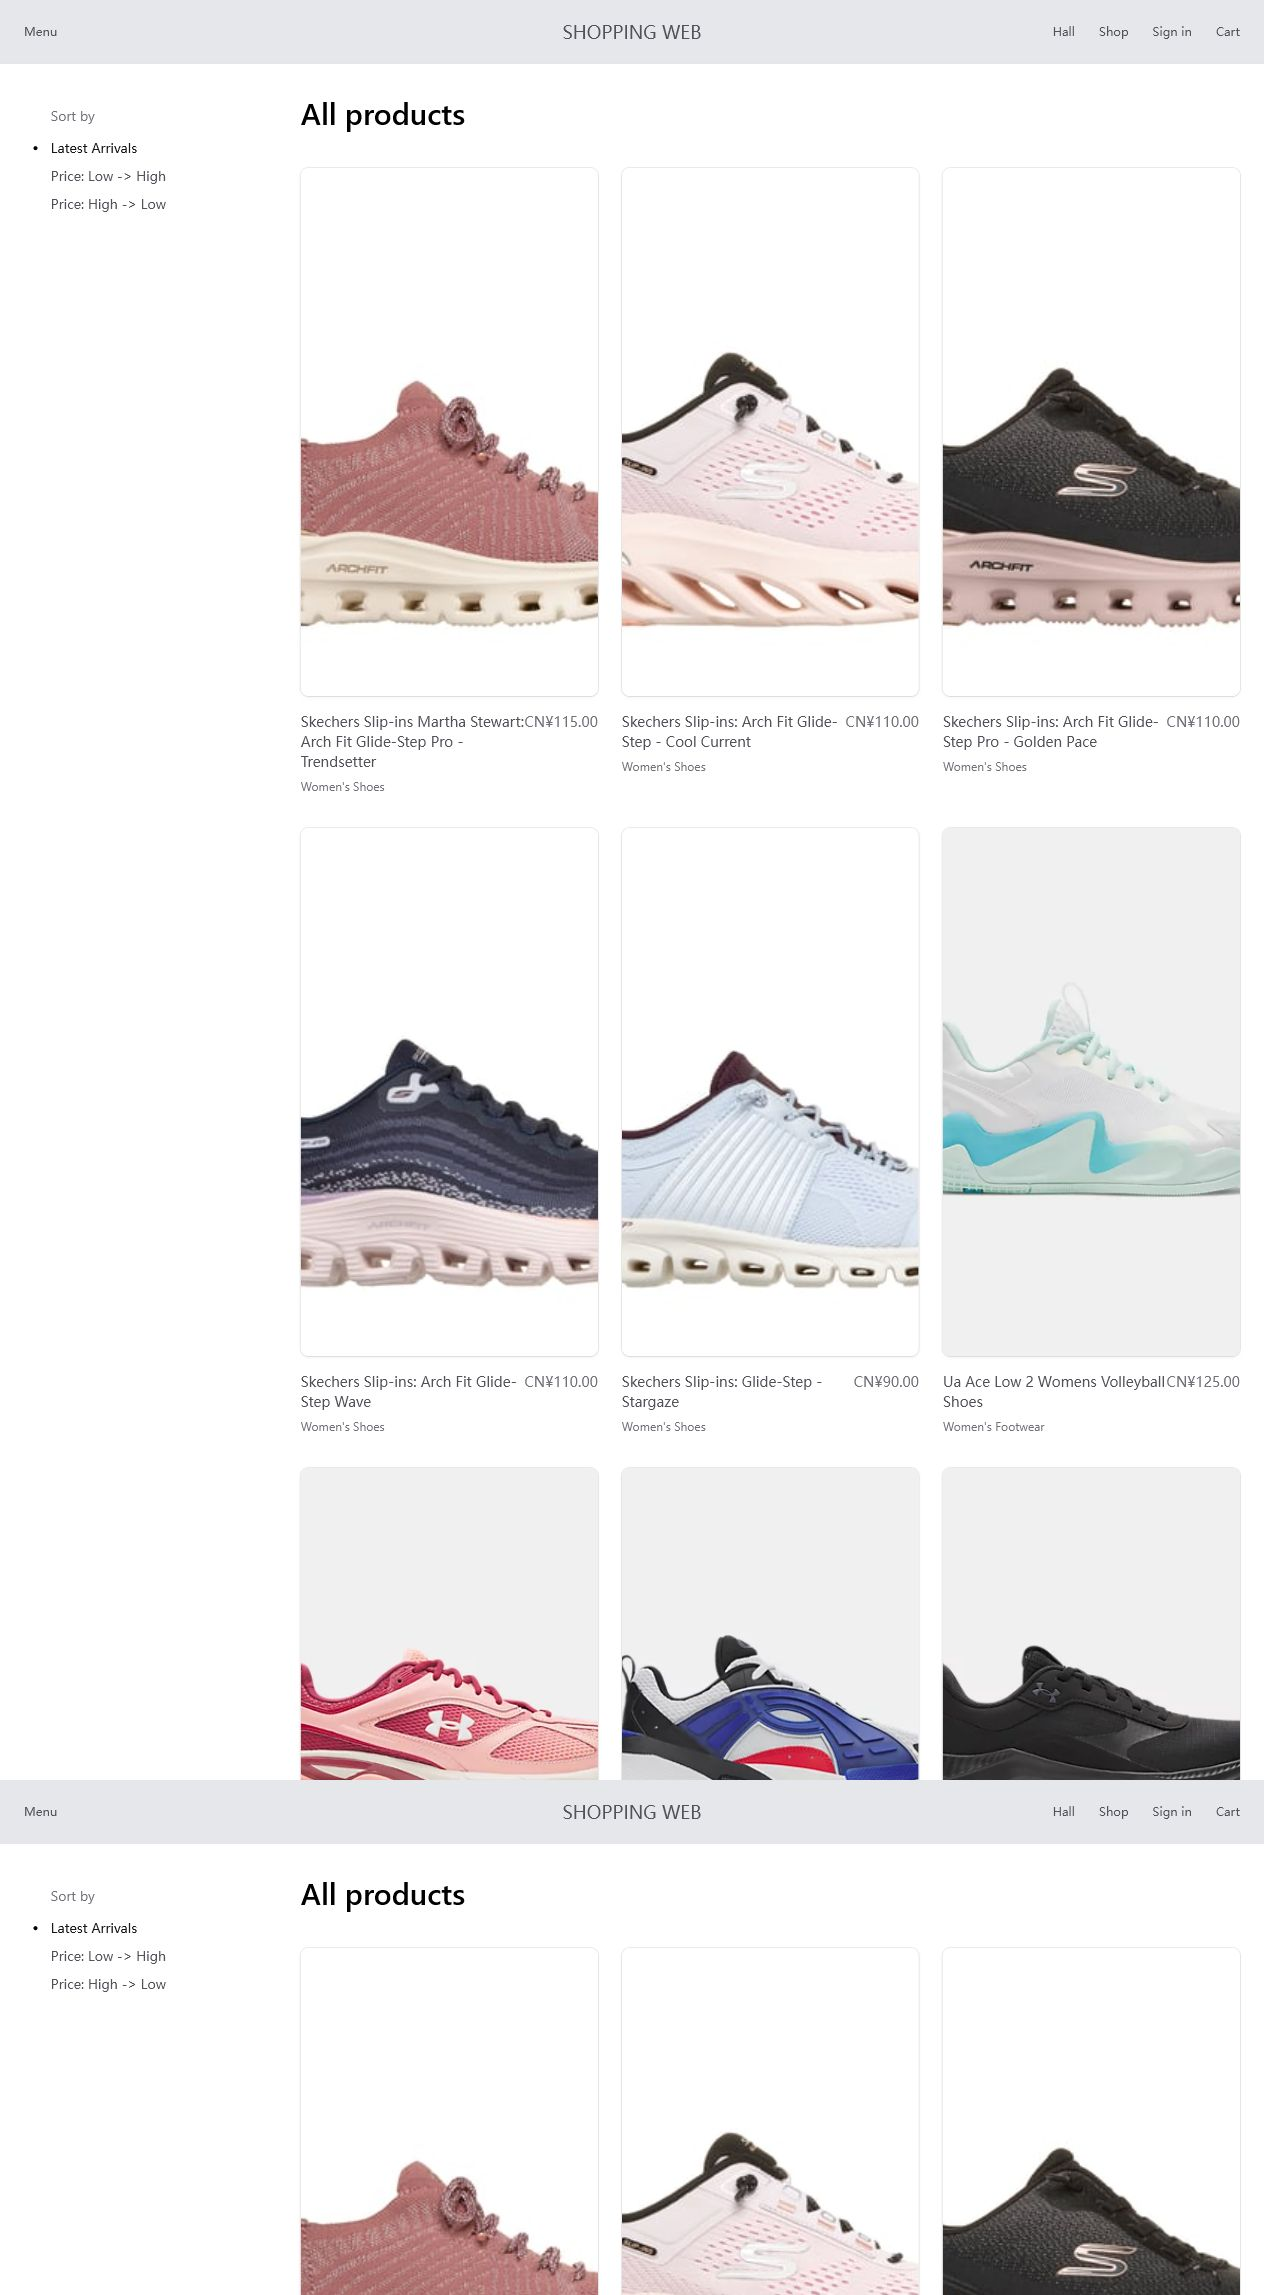
\includegraphics[width=0.92\textwidth,height=0.76\textheight,keepaspectratio]{implementation-shop-long.png}
  \caption{商品列表初始状态长截图}
  \label{fig:implementation_shop_long_extra}
\end{figure}

当客户输入关键字或携带搜索条件进入商品列表页时，系统会根据查询条件重新组织商品结果。搜索前后的变化主要体现在结果集范围缩小、列表内容更新和页面地址参数变化。前端根据搜索参数请求后端商品数据，后端完成关键字匹配和状态过滤，再把结果返回给页面展示。商品搜索结果如图 \ref{fig:implementation_shop_search} 所示。

\begin{figure}[H]
  \centering
  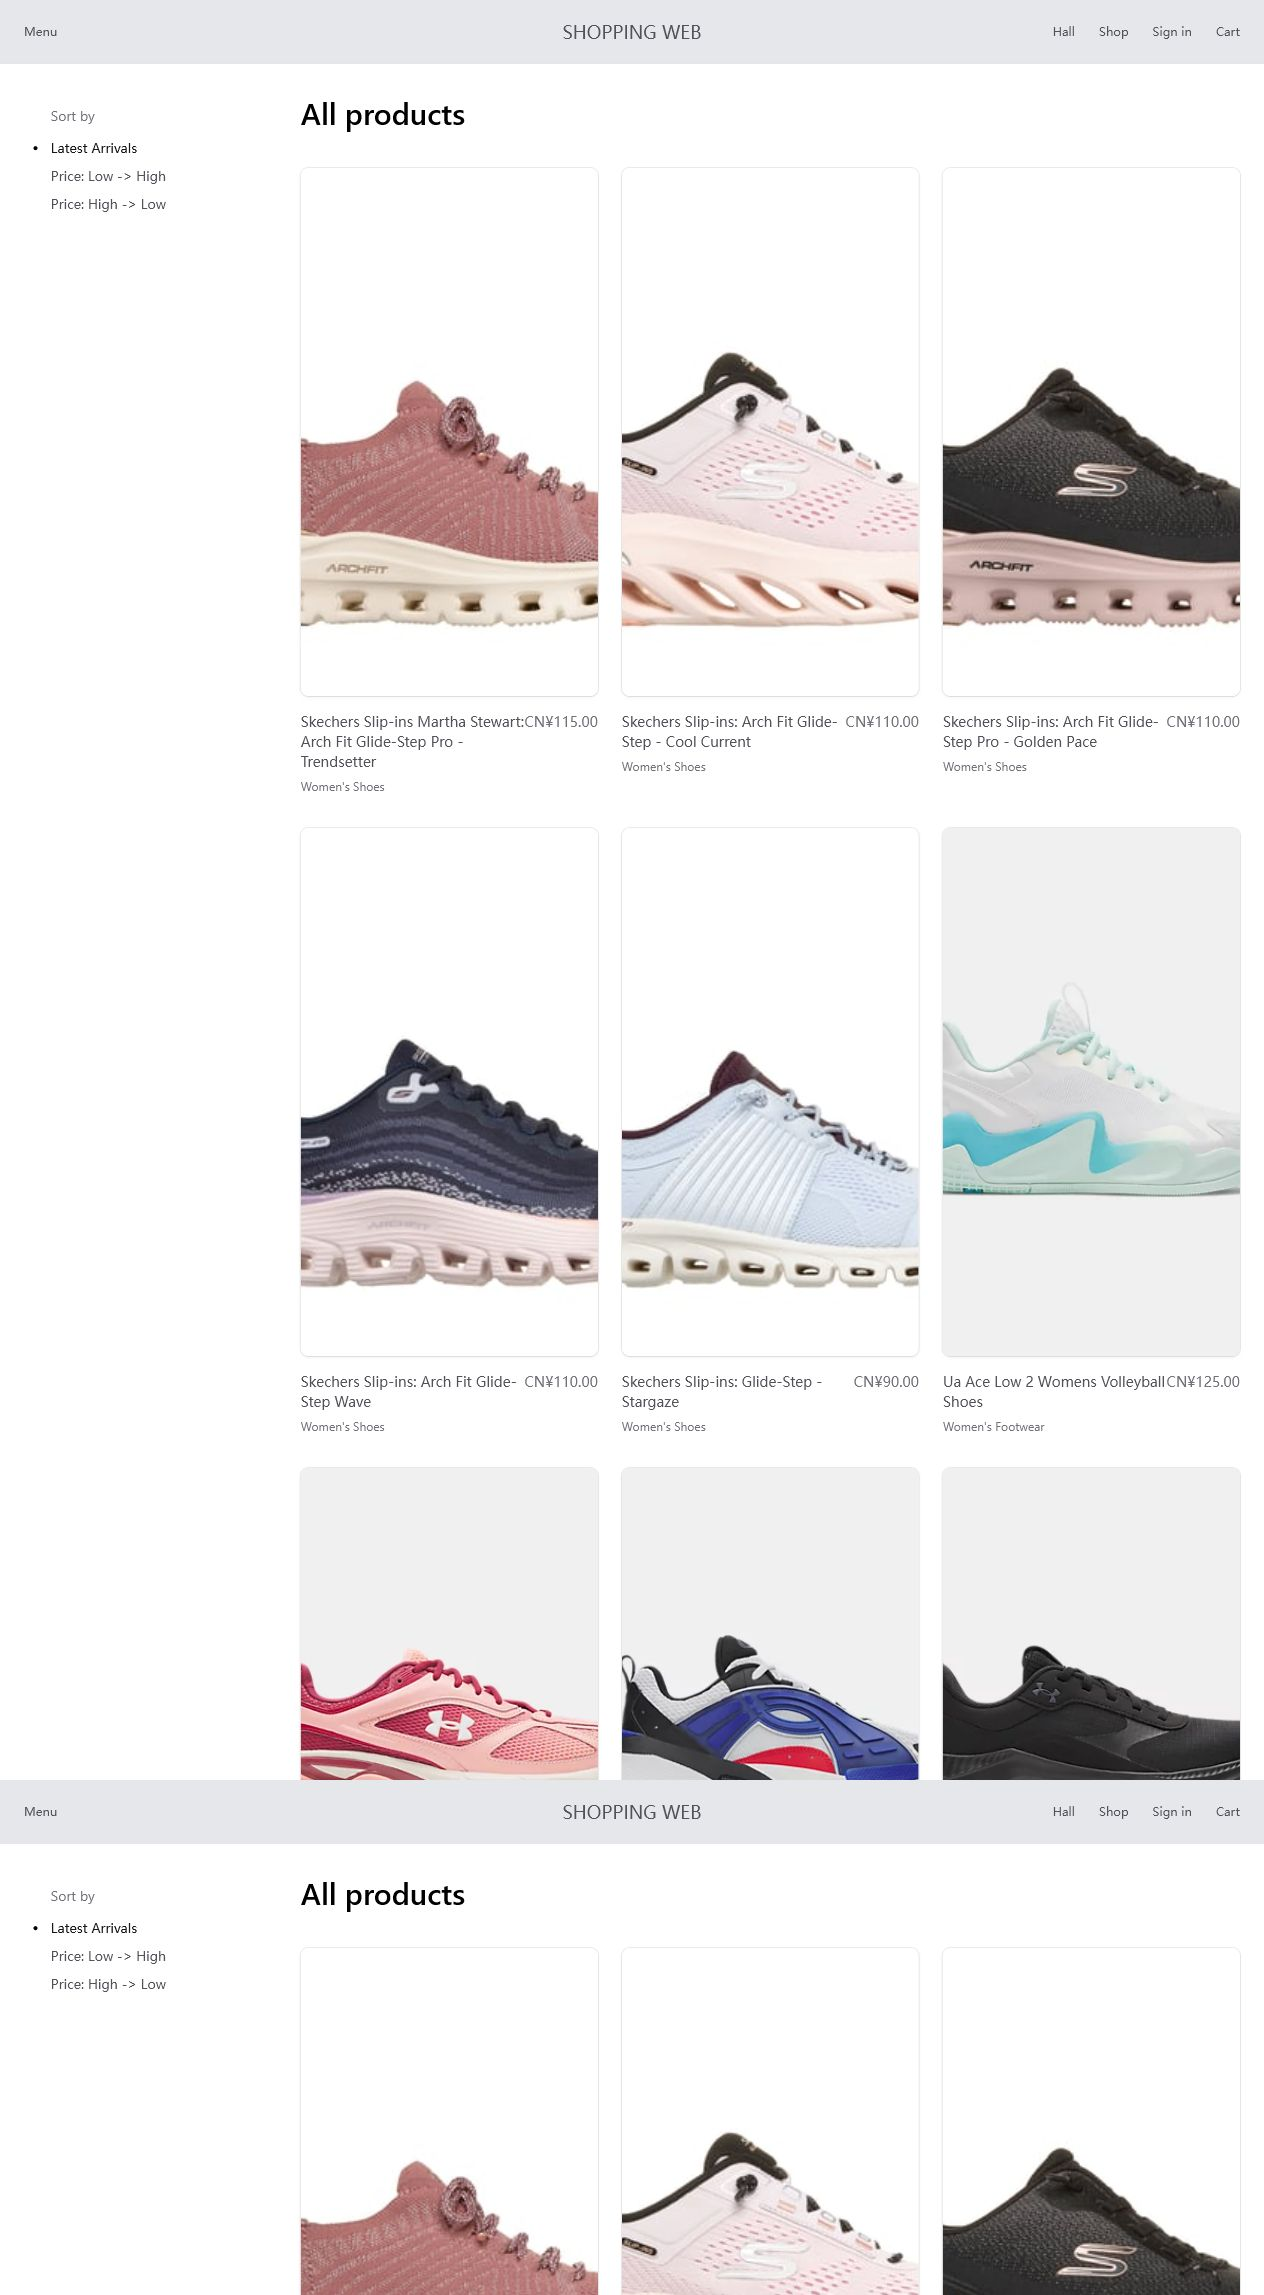
\includegraphics[width=0.92\textwidth,height=0.76\textheight,keepaspectratio]{implementation-shop-search-shoes-long.png}
  \caption{商品搜索结果长截图}
  \label{fig:implementation_shop_search}
\end{figure}

排序状态用于帮助客户按照价格、时间或其他规则重新比较商品。排序操作不会改变商品本身的数据，只改变结果展示顺序。该功能的实现重点是让排序条件能够被页面状态保存，并在刷新或跳转后仍能复现当前结果。商品排序后的页面状态如图 \ref{fig:implementation_shop_sort} 所示。

\begin{figure}[H]
  \centering
  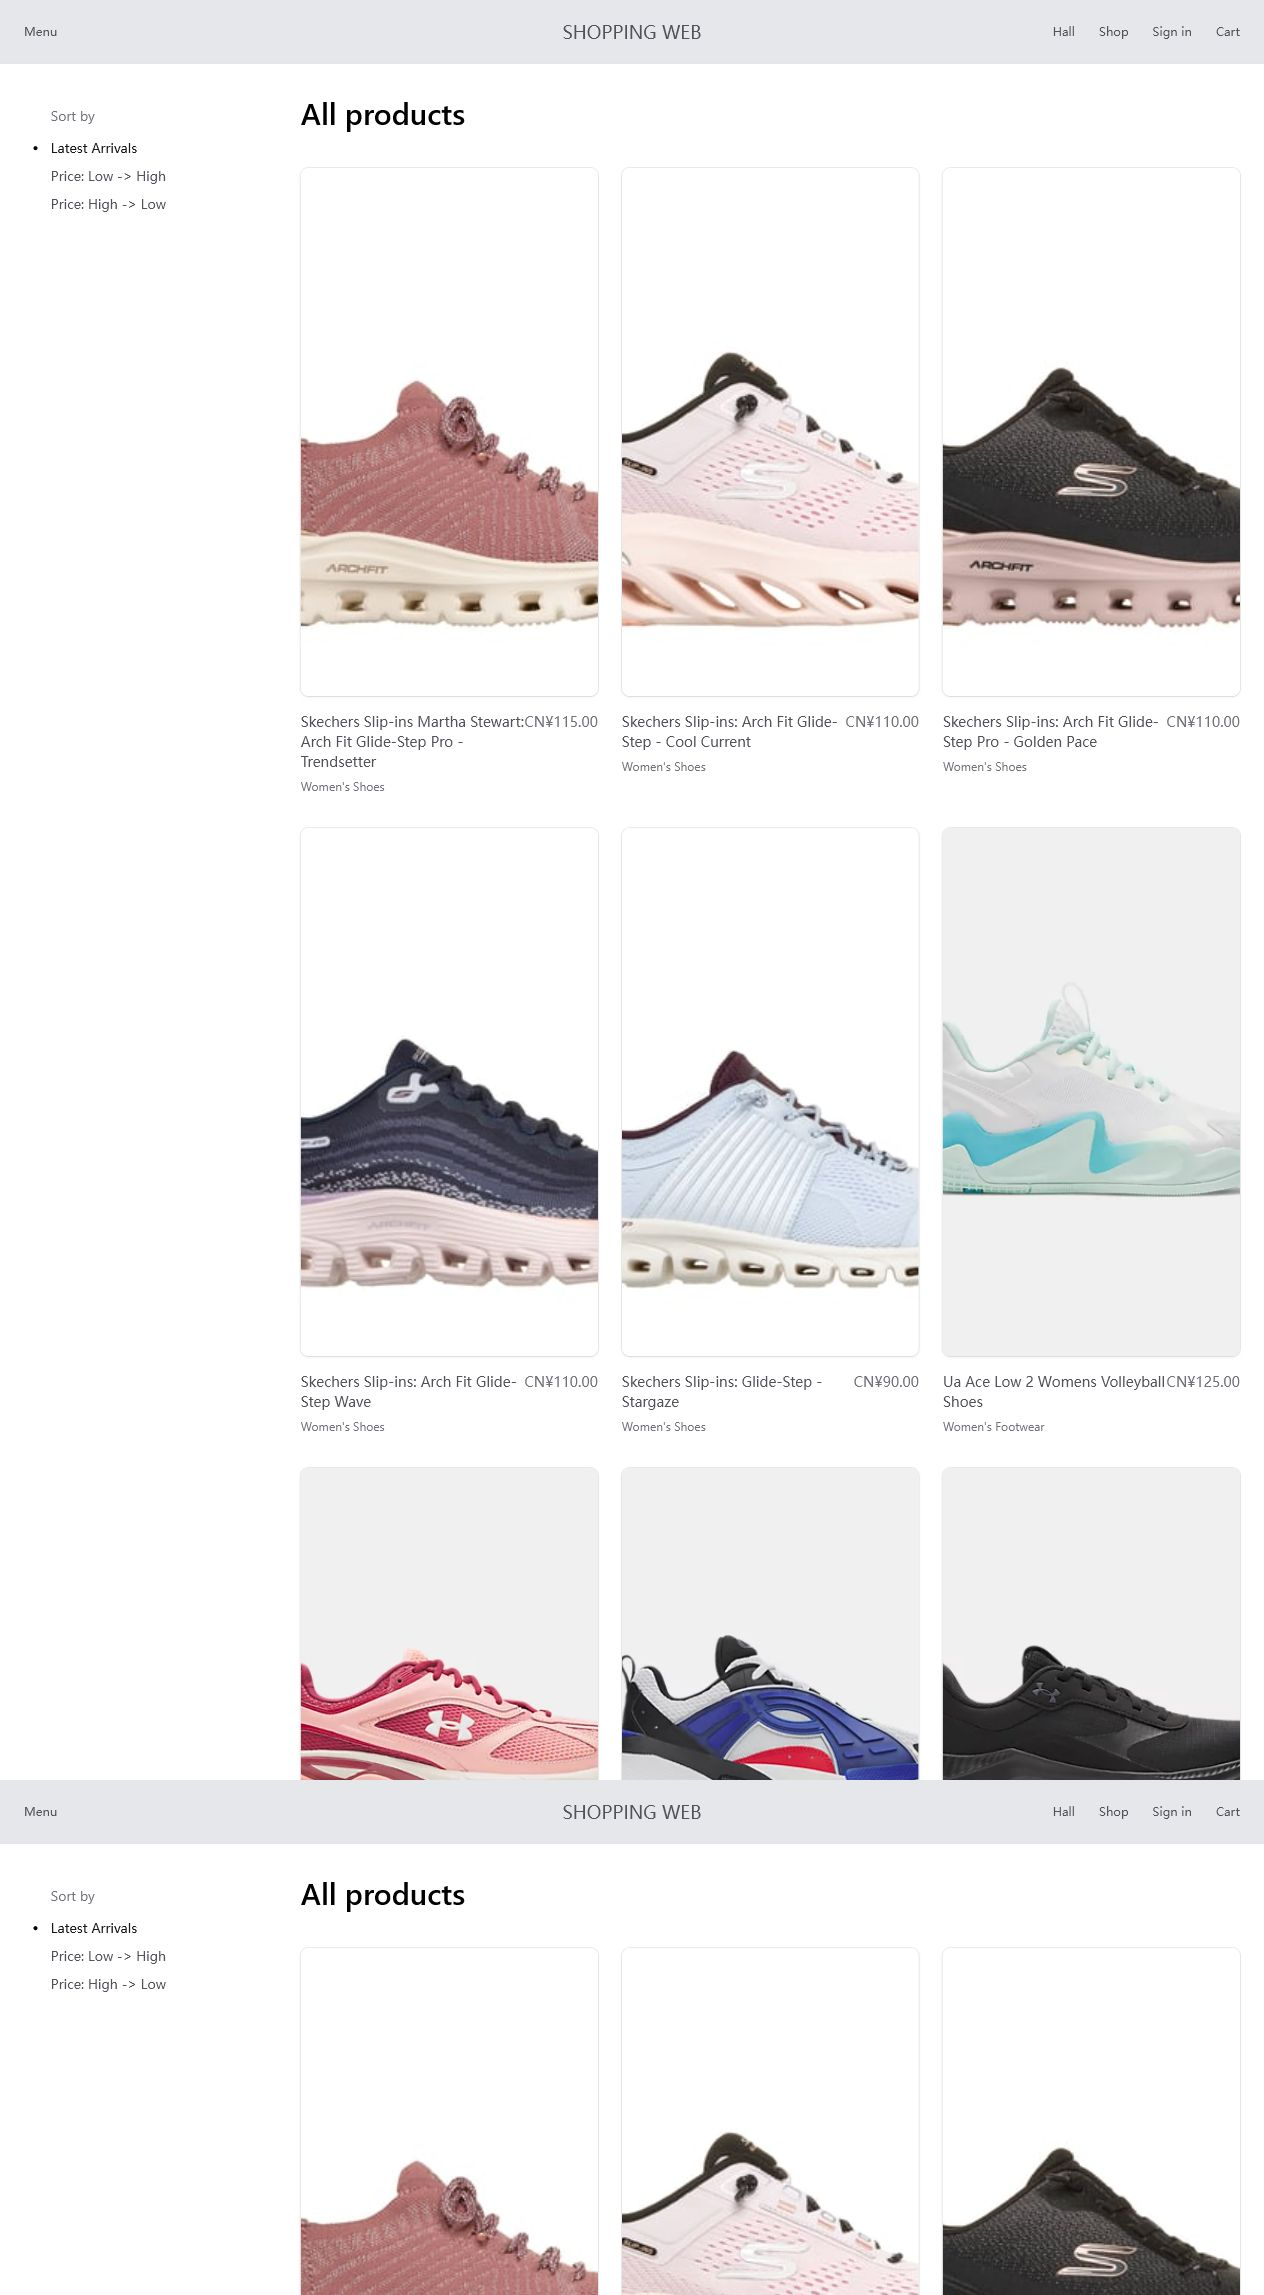
\includegraphics[width=0.92\textwidth,height=0.76\textheight,keepaspectratio]{implementation-shop-sort-price-long.png}
  \caption{商品排序结果长截图}
  \label{fig:implementation_shop_sort}
\end{figure}

店铺列表页用于从商家维度组织商品资源。客户可以先选择店铺，再查看该店铺下的商品集合。该页面展示了店铺名称、商品数量、分类摘要以及店铺内部分商品预览。与单纯商品列表相比，店铺列表更适合客户按品牌或经营主体进行浏览，也为商家经营能力提供展示窗口。店铺列表效果如图 \ref{fig:implementation_shops} 所示。

\begin{figure}[H]
  \centering
  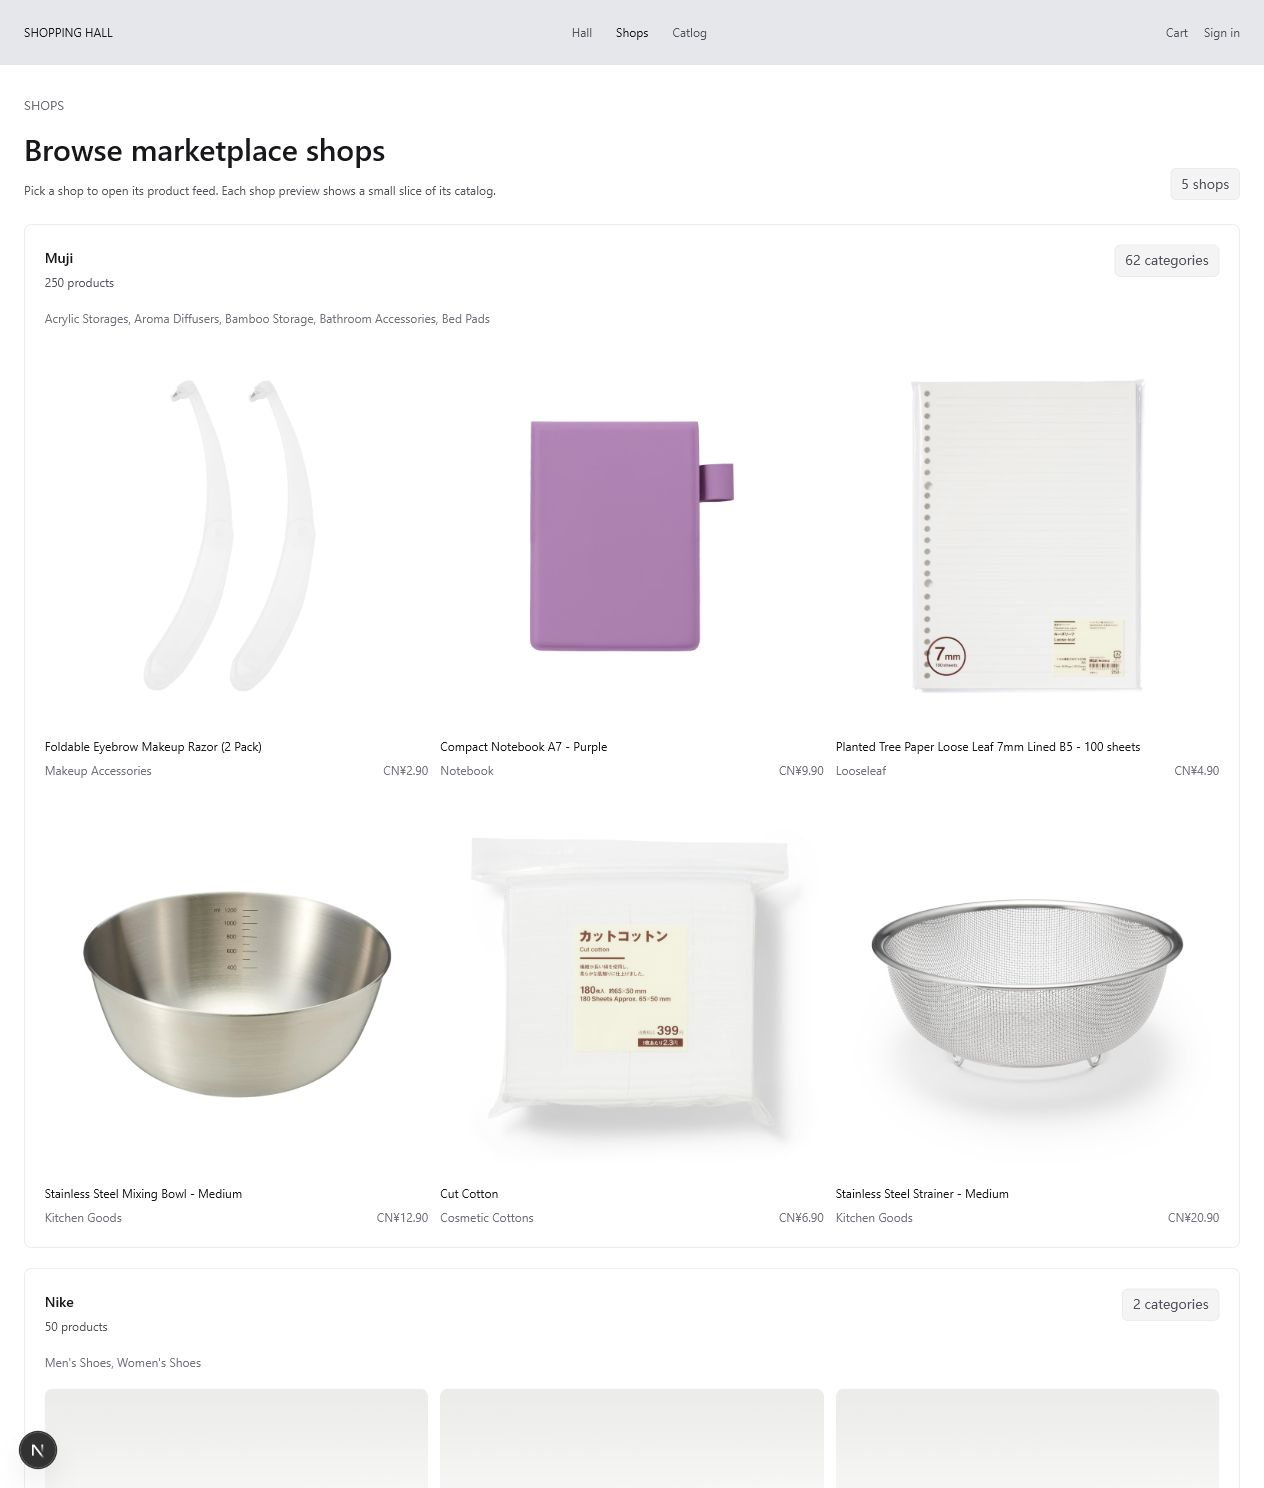
\includegraphics[width=0.92\textwidth,height=0.76\textheight,keepaspectratio]{implementation-shops-long.png}
  \caption{店铺列表长截图}
  \label{fig:implementation_shops}
\end{figure}

分类目录页用于从商品类别维度组织浏览入口。页面上方展示类别标签和统计信息，下方按照分类分组展示代表性商品。该页面能够帮助客户快速理解商城商品结构，并从高频类别进入对应商品集合。分类目录页还可以作为推荐和筛选之间的过渡页面，使客户不必完全依赖关键字搜索。分类目录效果如图 \ref{fig:implementation_catalog} 所示。

\begin{figure}[H]
  \centering
  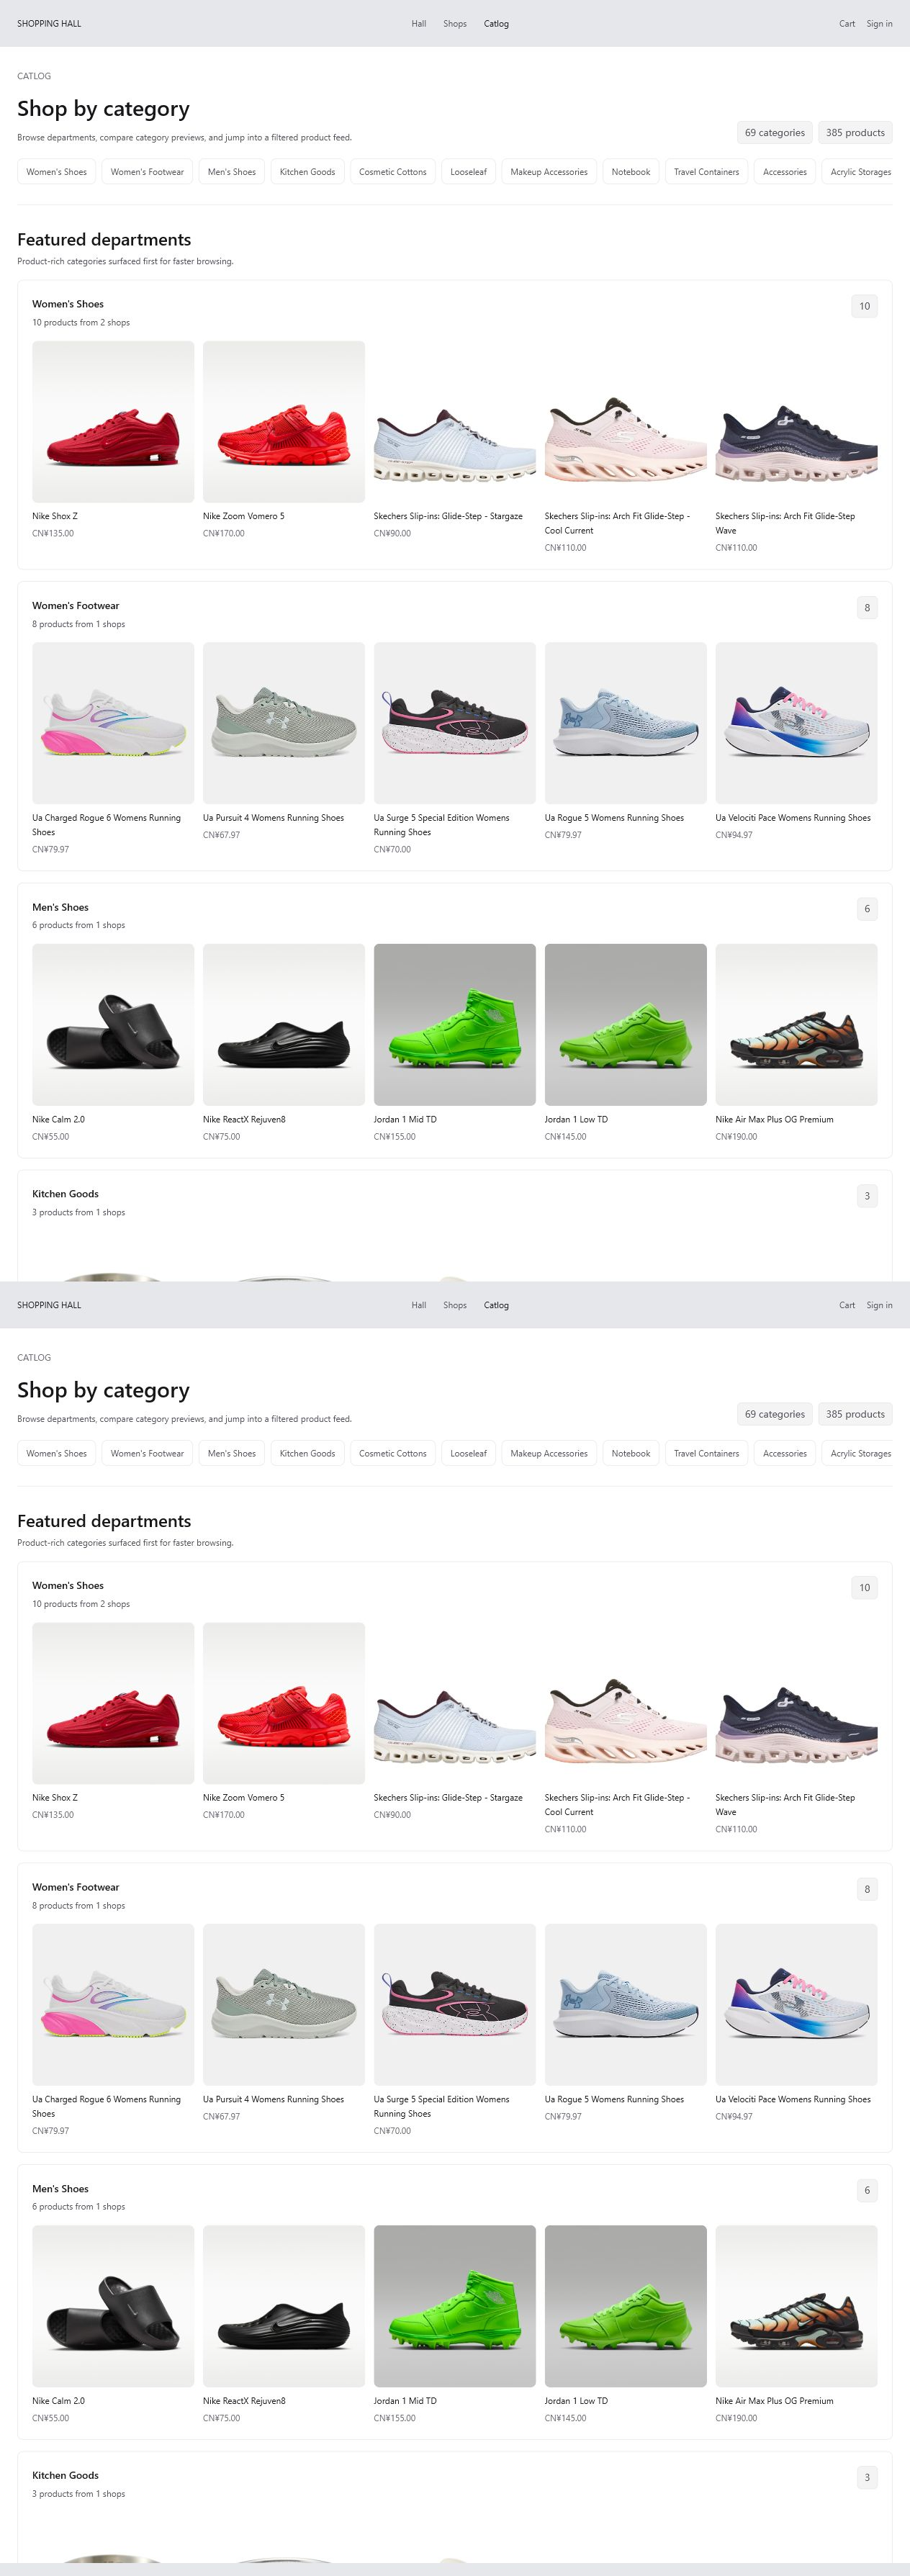
\includegraphics[width=0.92\textwidth,height=0.76\textheight,keepaspectratio]{implementation-catalog-long.png}
  \caption{分类目录长截图}
  \label{fig:implementation_catalog}
\end{figure}

购物车页面体现了购买流程中的中间状态。当前截图展示空购物车状态，系统在没有商品时给出继续浏览商品的入口。空状态不是异常状态，而是购物车模块必须覆盖的正常场景。若购物车中存在商品，页面应展示商品明细、数量调整、价格小计和进入结算的操作；若购物车为空，则应引导客户回到商品浏览路径。购物车空状态如图 \ref{fig:implementation_cart_long_extra} 所示。

\begin{figure}[H]
  \centering
  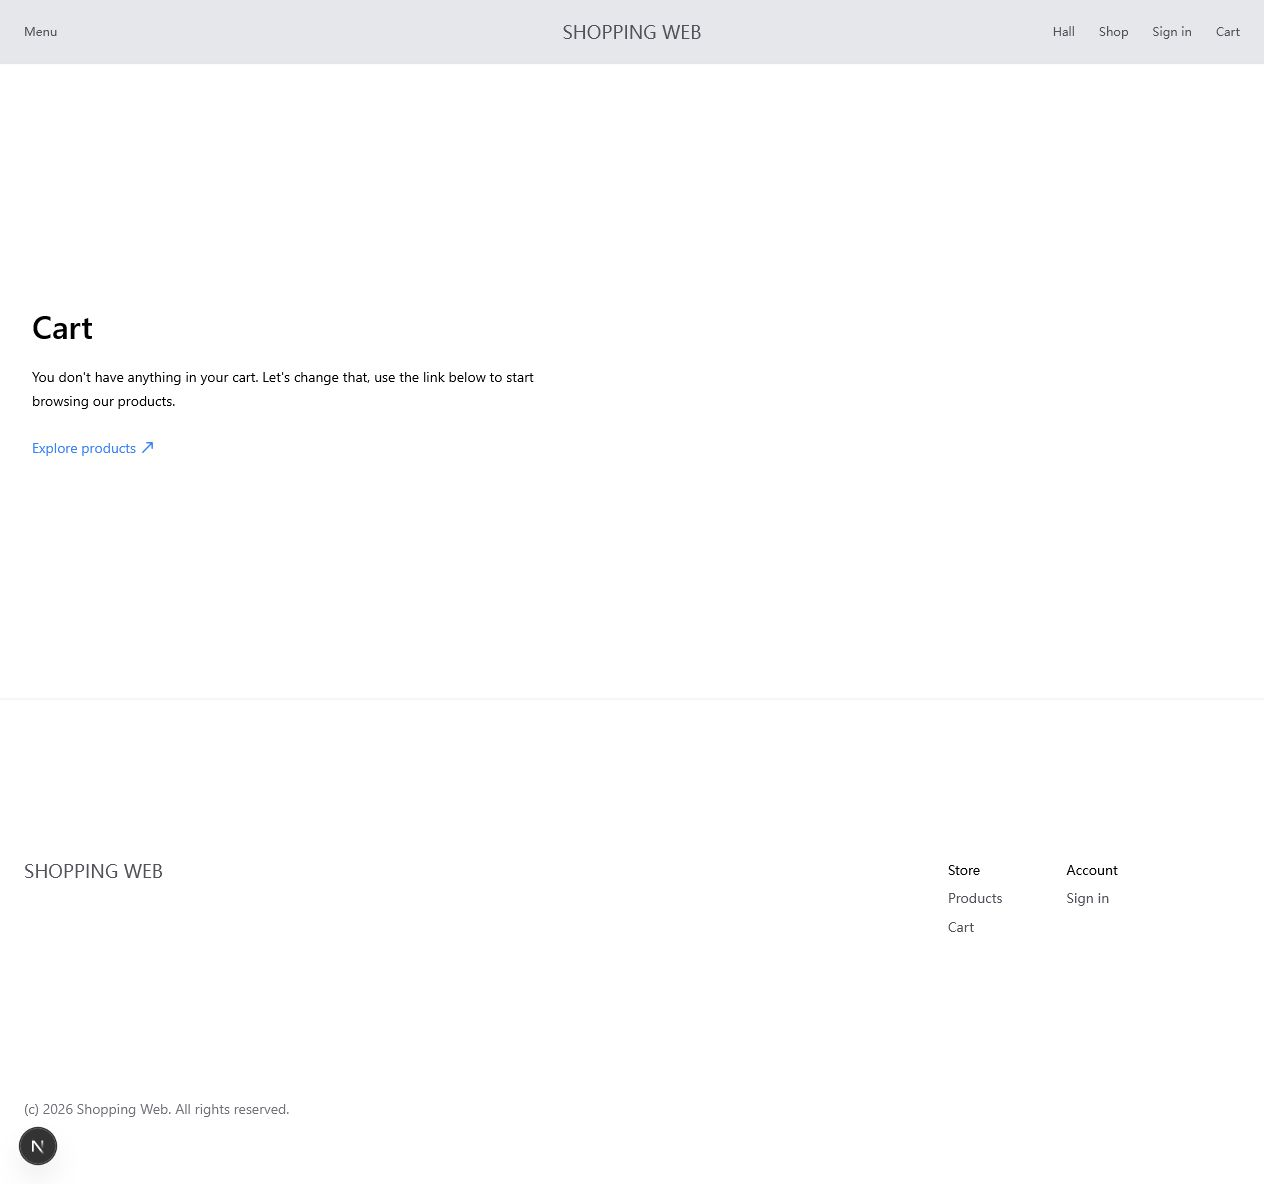
\includegraphics[width=0.92\textwidth,height=0.76\textheight,keepaspectratio]{implementation-cart-long.png}
  \caption{购物车空状态长截图}
  \label{fig:implementation_cart_long_extra}
\end{figure}

统一登录页展示客户、商家和管理员三类角色入口。页面通过角色卡片让用户先明确身份类型，再输入账户信息。不同角色共享认证流程，但认证通过后的目标页面和权限范围不同。该设计能够减少重复登录页面，也便于在后端统一进行账户状态校验、密码校验和角色校验。统一登录页如图 \ref{fig:implementation_login_long_extra} 所示。

\begin{figure}[H]
  \centering
  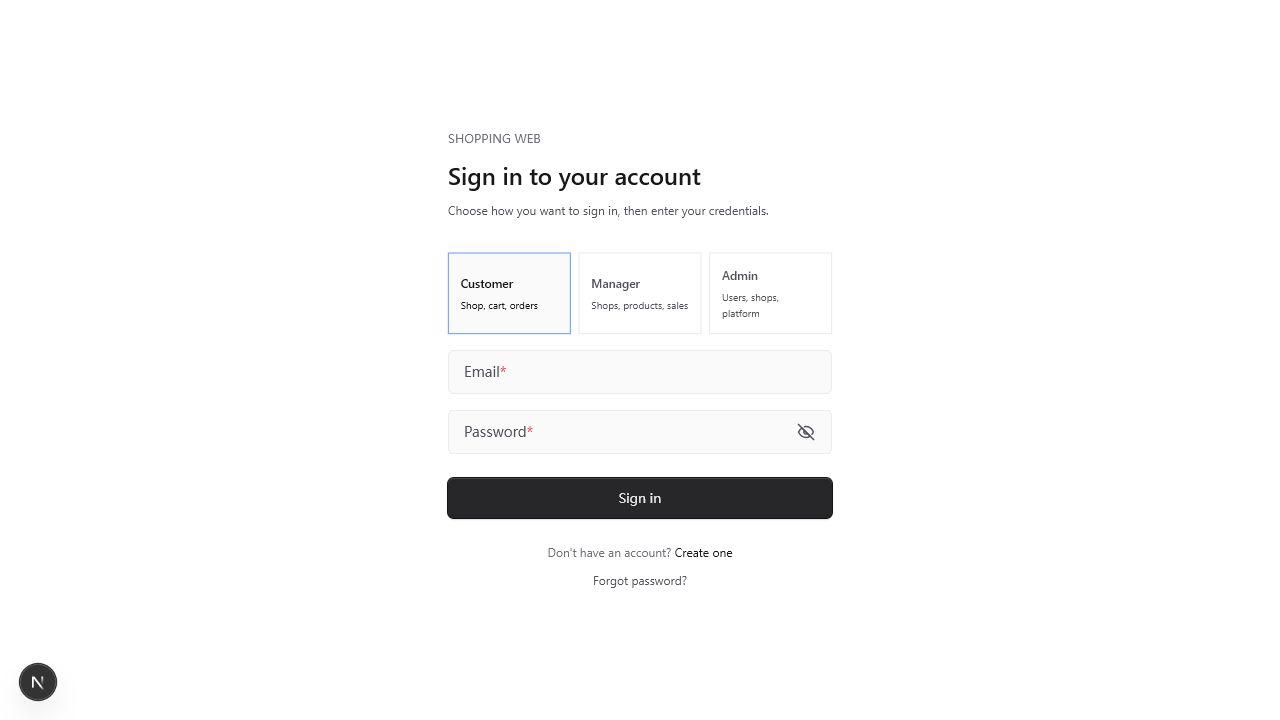
\includegraphics[width=0.86\textwidth,height=0.72\textheight,keepaspectratio]{implementation-login-long.png}
  \caption{统一登录页长截图}
  \label{fig:implementation_login_long_extra}
\end{figure}

系统还提供角色化登录入口。客户登录入口面向购物、订单和个人资料管理；商家登录入口面向店铺经营和商品维护；管理员登录入口面向审核和平台治理。虽然三个入口在视觉上保持统一，但在业务语义上分别对应不同的权限边界。角色入口页如图 \ref{fig:implementation_signin_roles} 所示。

\begin{figure}[H]
  \centering
  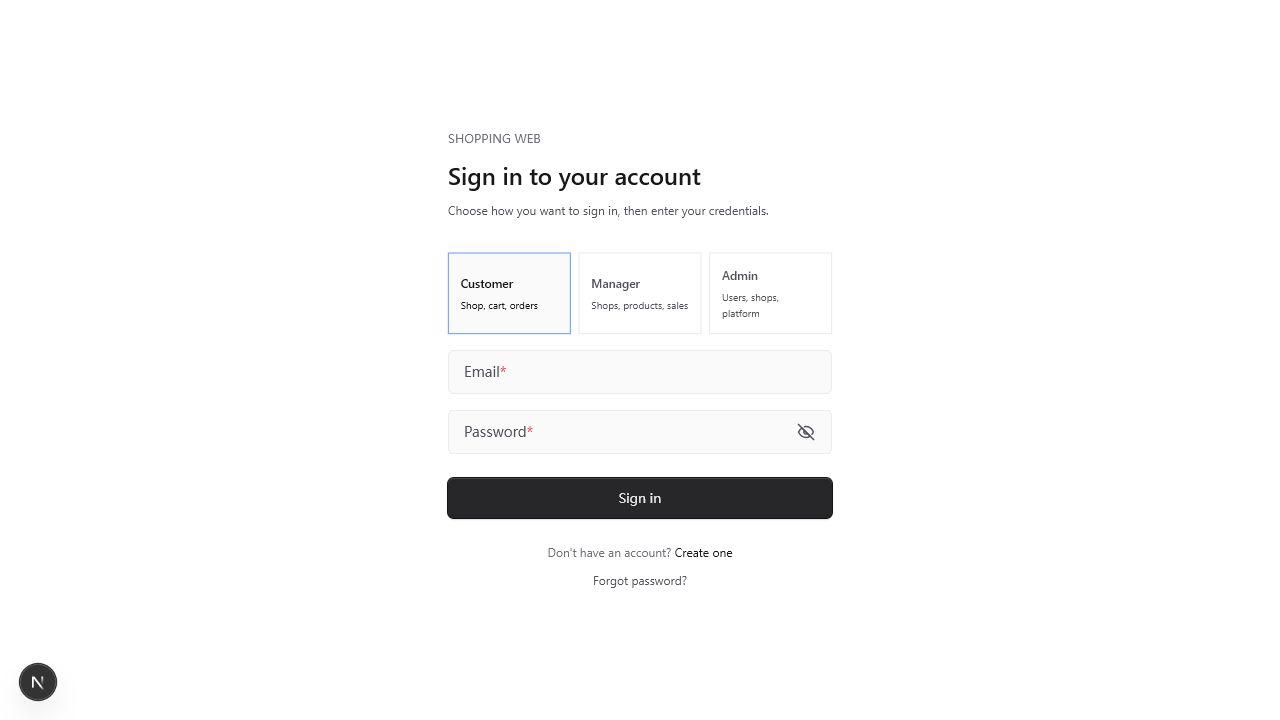
\includegraphics[width=0.86\textwidth,height=0.72\textheight,keepaspectratio]{implementation-signin-long.png}
  \caption{角色登录选择页长截图}
  \label{fig:implementation_signin_roles}
\end{figure}

客户、商家和管理员也可以从独立入口进入同一登录组件。独立入口的作用是让导航路径更加明确，例如客户从购物流程进入登录，商家从经营入口进入登录，管理员从后台入口进入登录。三个入口保留一致的表单结构和交互方式，降低维护成本。客户登录入口、商家登录入口和管理员登录入口分别如图 \ref{fig:implementation_signin_customer}、图 \ref{fig:implementation_signin_manager} 和图 \ref{fig:implementation_signin_admin} 所示。

\begin{figure}[H]
  \centering
  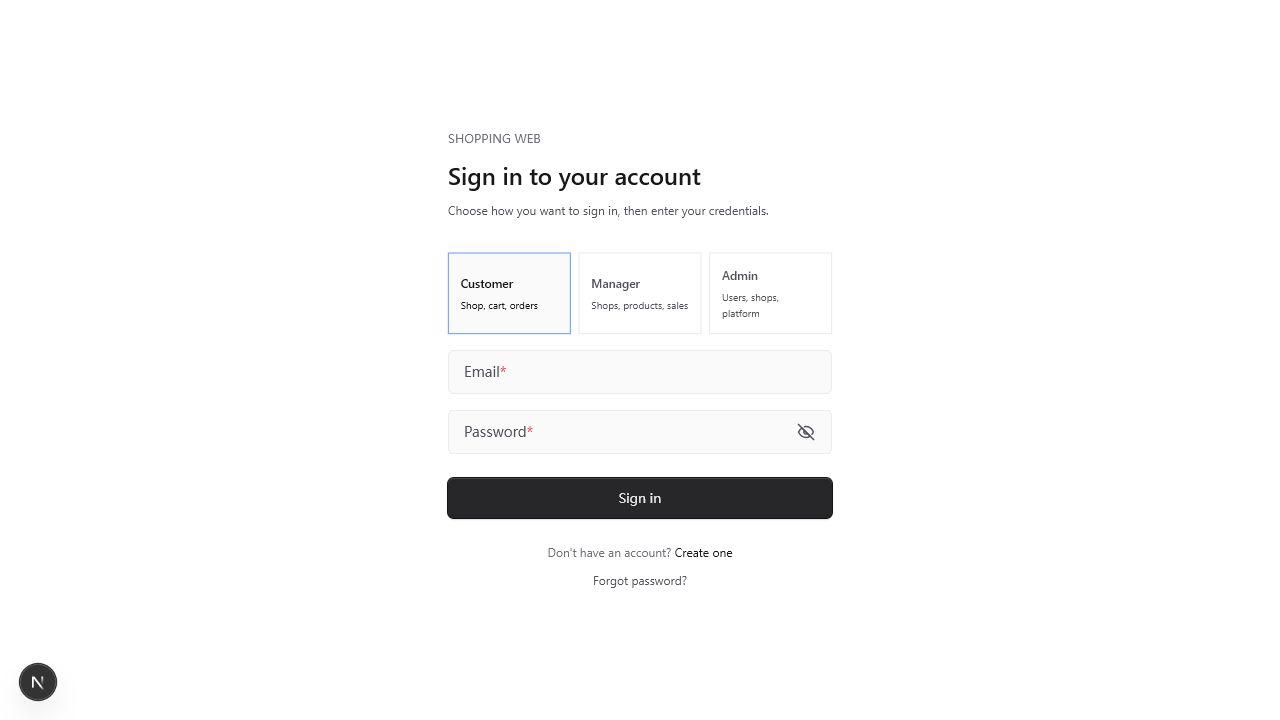
\includegraphics[width=0.86\textwidth,height=0.72\textheight,keepaspectratio]{implementation-signin-customer-long.png}
  \caption{客户登录入口长截图}
  \label{fig:implementation_signin_customer}
\end{figure}

\begin{figure}[H]
  \centering
  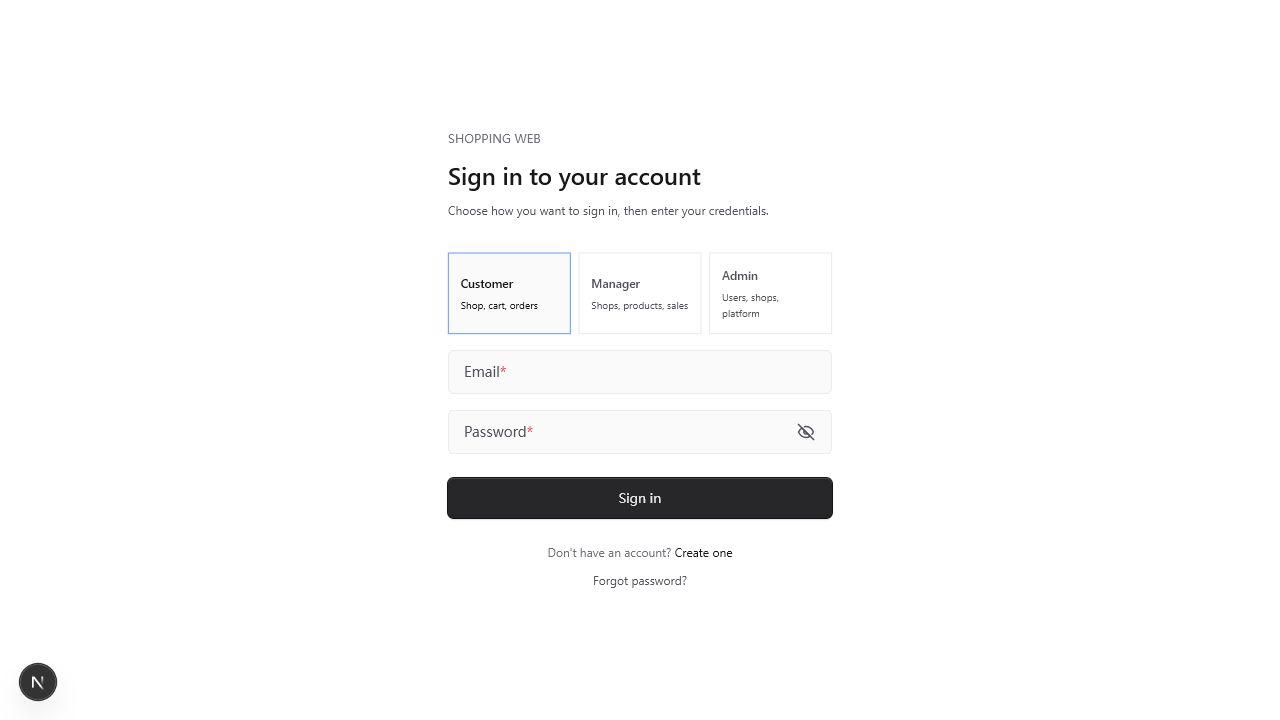
\includegraphics[width=0.86\textwidth,height=0.72\textheight,keepaspectratio]{implementation-signin-manager-long.png}
  \caption{商家登录入口长截图}
  \label{fig:implementation_signin_manager}
\end{figure}

\begin{figure}[H]
  \centering
  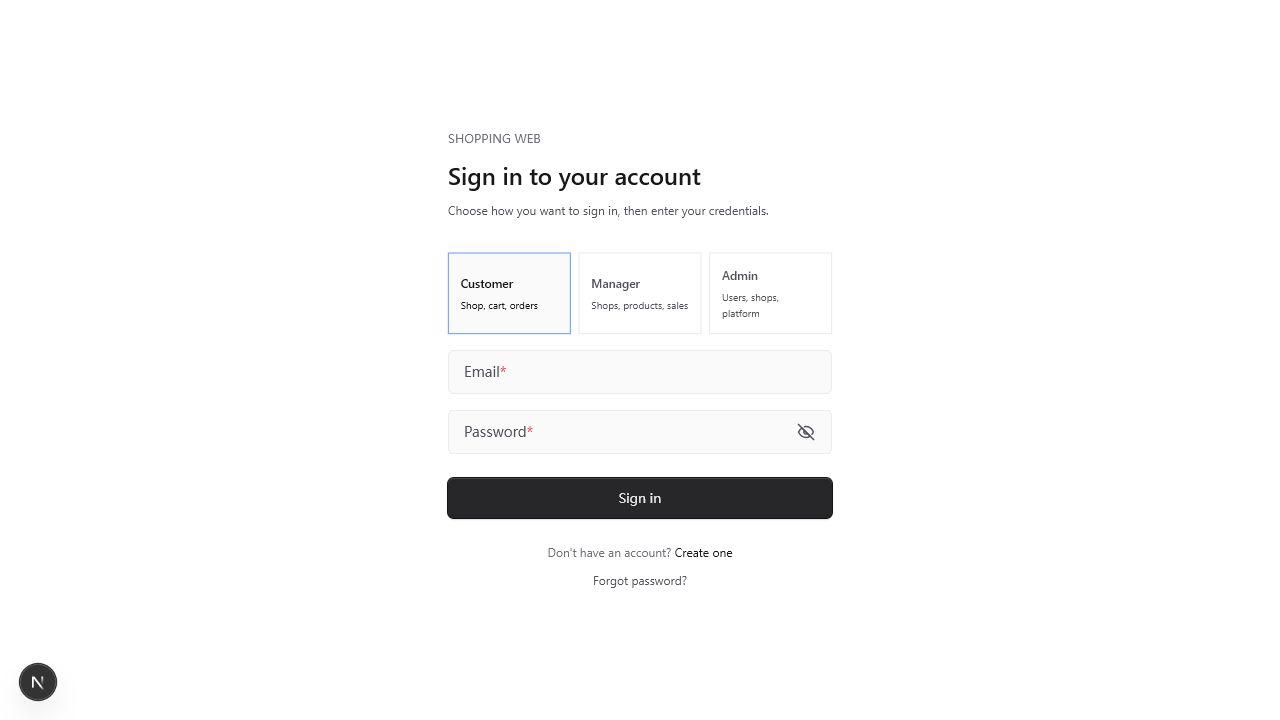
\includegraphics[width=0.86\textwidth,height=0.72\textheight,keepaspectratio]{implementation-signin-admin-long.png}
  \caption{管理员登录入口长截图}
  \label{fig:implementation_signin_admin}
\end{figure}

注册页面用于新用户创建账户。注册流程需要收集基本身份信息、联系方式、密码和角色类型，并在提交前进行必填项与格式校验。注册功能的实现重点是防止重复账户、弱密码和无效联系方式进入系统，同时为后续角色权限分配提供准确基础。注册页面效果如图 \ref{fig:implementation_register} 所示。

\begin{figure}[H]
  \centering
  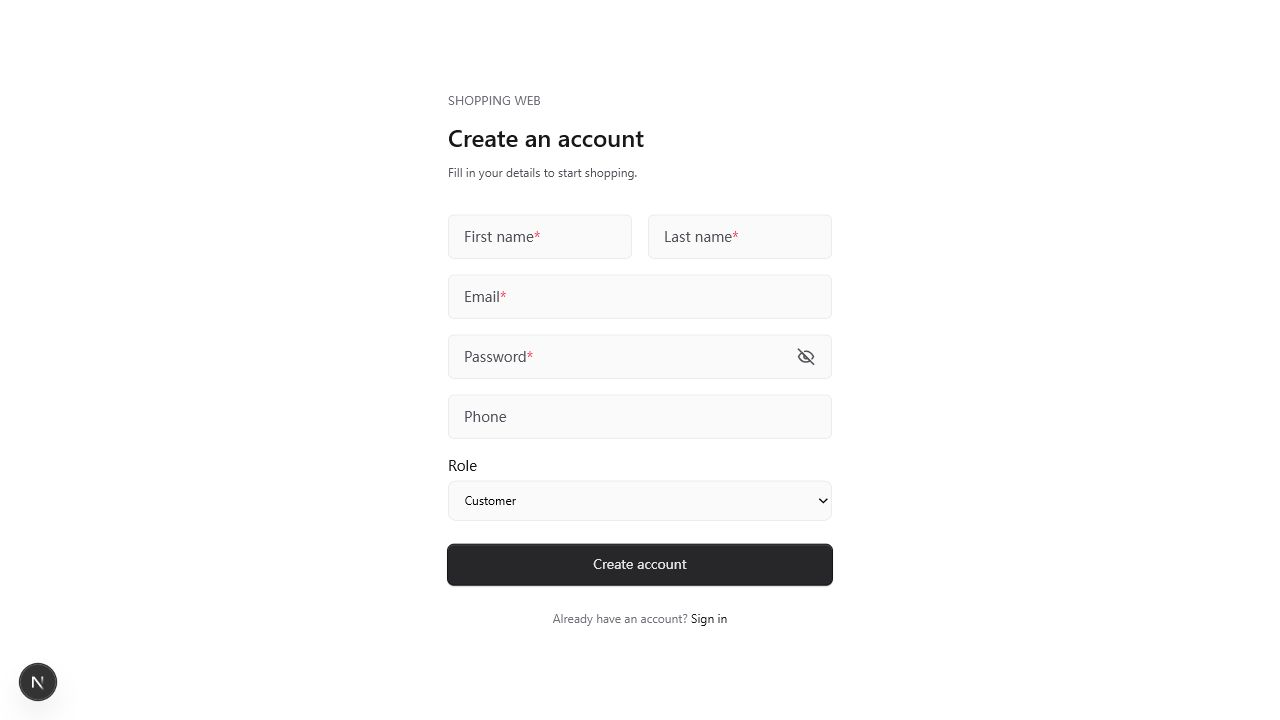
\includegraphics[width=0.86\textwidth,height=0.72\textheight,keepaspectratio]{implementation-register-long.png}
  \caption{账户注册页面长截图}
  \label{fig:implementation_register}
\end{figure}

找回密码页面用于处理用户忘记密码的情况。页面通过邮箱或账户信息定位用户，并引导后续重置流程。该页面属于账户安全辅助功能，虽然不直接参与购物交易，但对系统可用性和用户留存具有重要作用。找回密码页面如图 \ref{fig:implementation_forgot} 所示。

\begin{figure}[H]
  \centering
  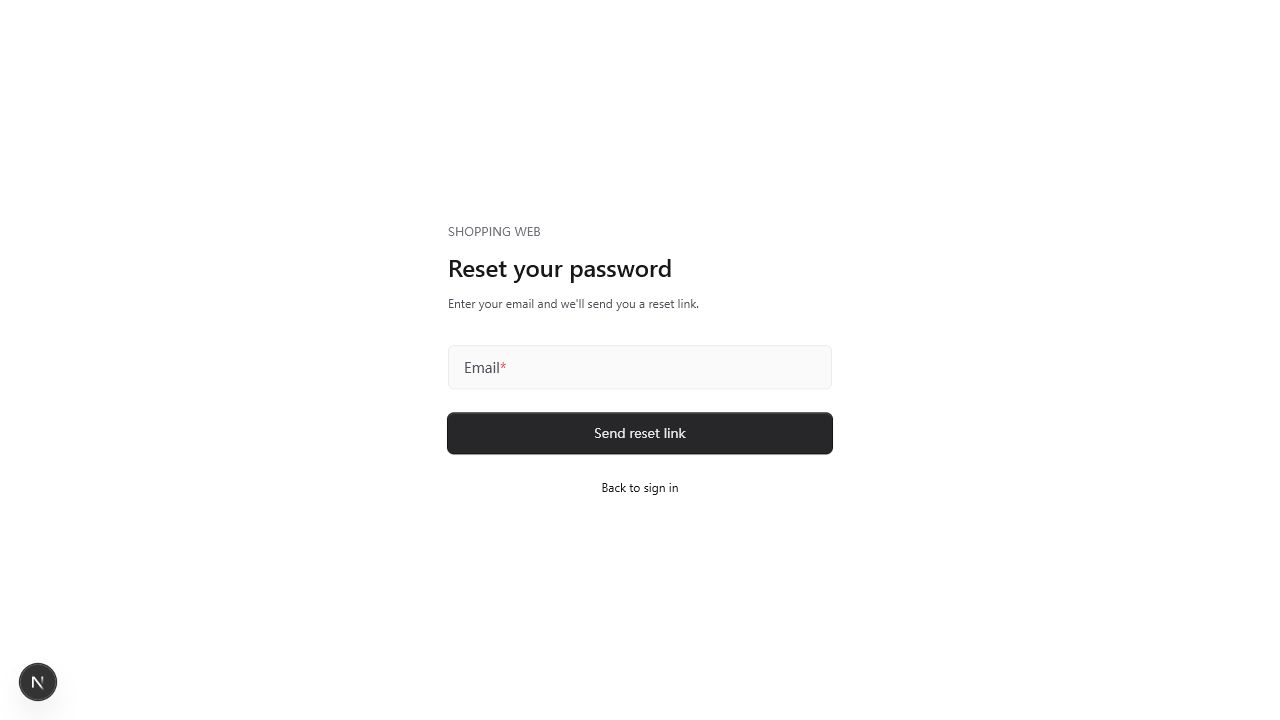
\includegraphics[width=0.86\textwidth,height=0.72\textheight,keepaspectratio]{implementation-forgot-long.png}
  \caption{找回密码页面长截图}
  \label{fig:implementation_forgot}
\end{figure}

客户中心入口用于承接客户登录后的个人功能，包括购物车、订单、支付、收藏、评价、资料和设置等。该入口把客户相关功能集中到一个导航结构中，使客户能够从购买前、购买中和购买后不同阶段查看自己的数据。客户中心入口如图 \ref{fig:implementation_customer_panel} 所示。

\begin{figure}[H]
  \centering
  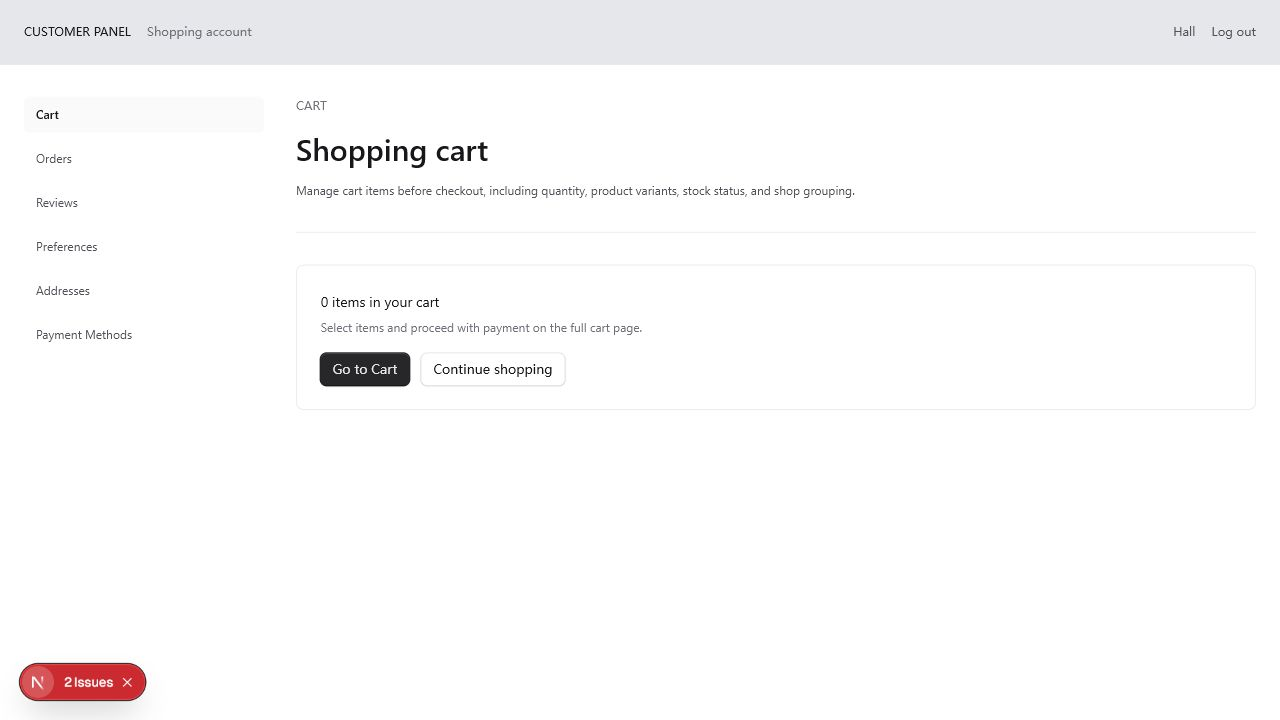
\includegraphics[width=0.88\textwidth,height=0.72\textheight,keepaspectratio]{implementation-customer-panel-long.png}
  \caption{客户中心入口长截图}
  \label{fig:implementation_customer_panel}
\end{figure}

商家仪表盘用于展示经营概览。页面左侧是商家后台导航，右侧展示店铺数量、商品数量、订单数量和收入等指标，并提供店铺申请、商品管理、订单管理、经营分析、收入统计和设置等入口。该页面体现了商家侧功能的组织方式：先展示经营状态，再引导商家进入具体管理动作。商家仪表盘如图 \ref{fig:implementation_manager_dashboard} 所示。

\begin{figure}[H]
  \centering
  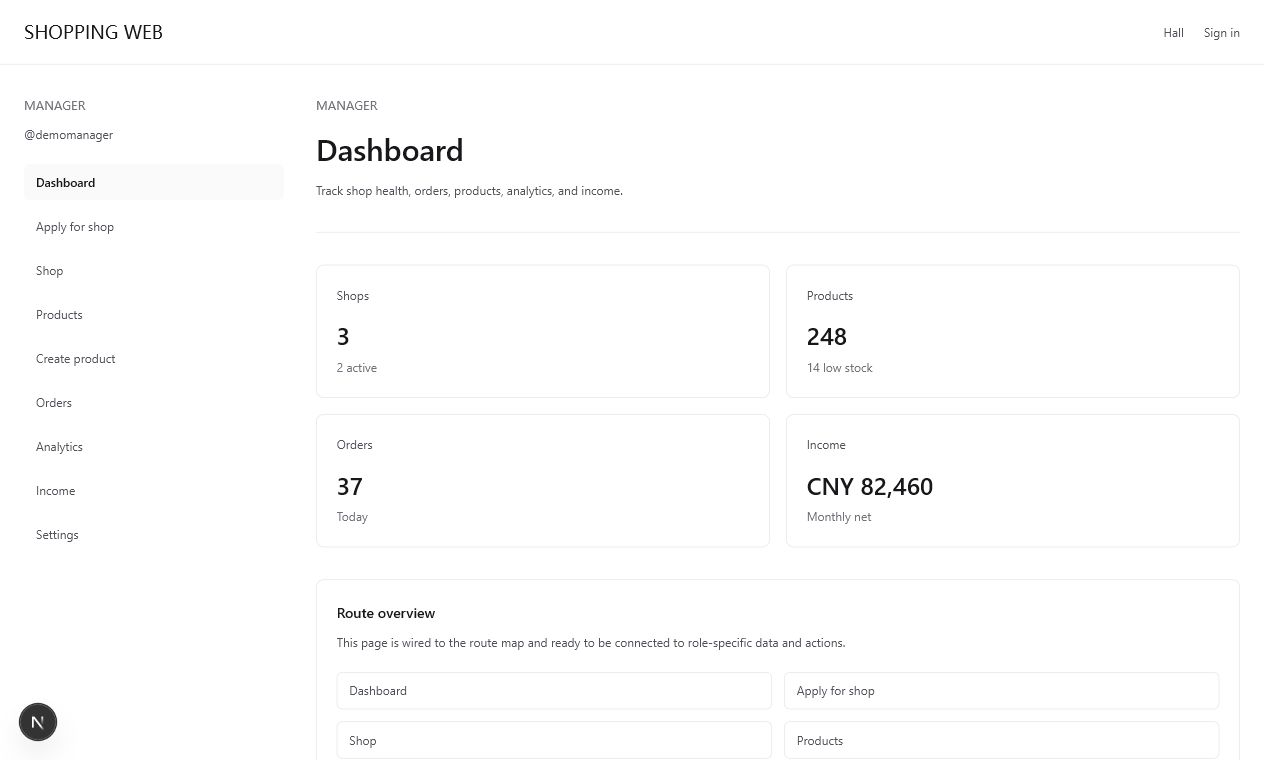
\includegraphics[width=0.92\textwidth,height=0.76\textheight,keepaspectratio]{implementation-manager-demo-dashboard-long.png}
  \caption{商家仪表盘长截图}
  \label{fig:implementation_manager_dashboard}
\end{figure}

从上述页面可以看出，系统页面实现遵循“入口清晰、状态明确、角色分离”的原则。客户侧页面强调浏览和购买路径，商家侧页面强调经营数据和管理入口，管理员侧功能在设计上强调审核、治理和平台状态控制。由于当前运行环境中部分后台子页面需要完整登录态或服务端上下文支持，正式正文仅选取能够稳定打开并反映功能结构的页面作为截图依据，避免将运行错误页作为实现效果展示。

综上，本系统实现围绕前后端分离、角色权限隔离、结构化数据管理和推荐增强展示展开。客户侧功能保证浏览和购买流程顺畅，商家侧功能保证店铺经营和订单处理可控，管理员侧功能保证平台治理和审核流程清晰。各模块通过统一接口和数据模型协作，既满足当前在线商城的基本业务需求，也为后续扩展优惠促销、售后服务、运营统计和更复杂推荐策略保留了空间。

\end{document}
